% Supplementary material for "Can language models forecast inductively?".
%
% This file holds every appendix section, with every table inlined and every
% reported table value written as a literal. Generated table sources under
% tables/ are retained only as provenance.
\appendix
\raggedbottom
% Keep appendix lists visually aligned with the text block rather than using the
% article class's comparatively deep default margins.
\setlist[itemize,1]{leftmargin=1.35em,labelsep=.45em}
\setlist[enumerate,1]{leftmargin=1.55em,labelsep=.45em}
%============================================================================
% BEGIN appendix_guide.tex
%============================================================================
\section*{Appendices}
\pdfbookmark[1]{Appendices}{appendix-guide}

The appendices document the experimental designs, analyses, and supplementary results.
Appendix~\ref{app:carnival-coin-probe} describes the coin-flip illustration in Figure~\ref{fig:world-knowledge-evidence}.
Appendices~\ref{app:exp1}--\ref{app:exp4} present the methods and results for Experiments~1--4: forecast updating, contextual relationship selection, controlled transfer, and historical-market forecasting.
Appendix~\ref{app:exp3-complete-training-setup} gives the shared training configuration for Experiments~3--4.

% Every entry below is derived from its \label: \ref* supplies the number,
% \nameref* the heading text, and \pageref* the page. Nothing here is typed by
% hand, so the guide cannot drift out of sync with the appendix headings the way
% a hard-coded list does. Adding or reordering an appendix section only requires
% adding its label to the list.
\begingroup
\hypersetup{hidelinks}
\small
\setlength{\parskip}{0pt}
\makeatletter
\newcommand{\appendixguidechapter}[1]{%
  \par\addvspace{0.45\baselineskip}%
  \noindent\hyperref[#1]{\textbf{\makebox[2.8em][l]{\ref*{#1}}\nameref*{#1}}}%
  \nobreak\hfill\nobreak
  \hyperref[#1]{\textbf{\pageref*{#1}}}\par
}
\newcommand{\appendixguidesection}[1]{%
  \@dottedtocline{2}{1.3em}{3.4em}%
    {\hyperref[#1]{\numberline{\ref*{#1}}\nameref*{#1}}}%
    {\hyperref[#1]{\pageref*{#1}}}%
}
\makeatother

\appendixguidechapter{app:carnival-coin-probe}

\appendixguidechapter{app:exp1}
\appendixguidesection{app:exp1-sample}
\appendixguidesection{app:exp1-protocol}
\appendixguidesection{app:metrics}
\appendixguidesection{app:exp1-limitations}
\appendixguidesection{app:exp1-context-reversal}
\appendixguidesection{app:exp1-fresh-factorial}
\appendixguidesection{app:exp1-ladder}

\appendixguidechapter{app:coin-city}
\appendixguidesection{app:coin-city-design}
\appendixguidesection{app:coin-city-arms}
\appendixguidesection{app:coin-city-execution}
\appendixguidesection{app:coin-city-analysis}
\appendixguidesection{app:coin-city-results}
\appendixguidesection{app:coin-city-reference-selection}
\appendixguidesection{app:coin-city-mechanistic-probe}
\appendixguidesection{app:coin-city-robustness}
\appendixguidesection{app:coin-city-limitations}

\appendixguidechapter{app:exp3}
\appendixguidesection{app:exp3-coin-structural}
\appendixguidesection{app:exp3-eight-seed}
\appendixguidesection{app:exp3-learnability}
\appendixguidesection{app:exp3-evidence-use}
\appendixguidesection{app:exp3-shuffled-control}

\appendixguidechapter{app:exp4}
\appendixguidesection{app:exp3b-results}
\appendixguidesection{app:exp4-scale}
\appendixguidesection{app:exp4-price-ablation}

\appendixguidechapter{app:exp3-complete-training-setup}

\endgroup

\clearpage
\section{Descriptive coin-flip forecast elicitation}
\label{app:carnival-coin-probe}

Figure~\ref{fig:world-knowledge-evidence} illustrates a simple forecasting problem: predicting the next flip of an unfamiliar coin after observing two heads.
We elicited eight independent forecasts from each of GPT-5.4, Claude Opus~4.8, and DeepSeek V4-Pro at temperature $0.7$ with a 600-token output limit.
All 24 responses contained a parseable probability.
Each model marker in Figure~\ref{fig:world-knowledge-evidence} shows its eight-call mean, and the displayed $\approx .68$ value rounds the pooled mean of $.679$.
This descriptive probe is separate from Experiments~1--4.

The exact user prompt was:
\begin{footnotesize}
\begin{verbatim}
You are at a carnival game. A coin you have never seen before is flipped
twice in front of you, and it comes up heads both times. These two flips
are everything you know about this coin.

What is the probability that the next flip comes up heads?

Think about it intuitively, the way you actually would in the
moment -- do NOT use any formula, rule, or calculation, and do not
work out any numbers in your reasoning. Just reason in plain words
about what you'd expect and why. Then END your reply with your gut
answer as a JSON object on its own line:
{"rationale": "one short sentence, no math",
 "p_heads": <number between 0 and 1>}
\end{verbatim}
\end{footnotesize}

\begin{center}
\begin{minipage}{0.78\linewidth}
\centering
\captionof{table}{Forecasts underlying the three model markers in Figure~\ref{fig:world-knowledge-evidence}. Each row summarizes eight independent temperature-$0.7$ calls.}
\label{tab:carnival-coin-probe}
\small
\begin{tabular}{lccc}
\toprule
Model & Mean & Median & Range \\
\midrule
GPT-5.4 & $.644$ & $.670$ & $[.60,.67]$ \\
Claude Opus~4.8 & $.681$ & $.675$ & $[.65,.75]$ \\
DeepSeek V4-Pro & $.712$ & $.750$ & $[.60,.75]$ \\
\midrule
Pooled ($n=24$) & $.679$ & $.670$ & $[.60,.75]$ \\
\bottomrule
\end{tabular}
\end{minipage}
\end{center}

The probe contains no matched control condition.
The prompt describes an unfamiliar carnival coin and requests intuitive reasoning without calculation, so the observed forecasts cannot distinguish the effect of the carnival context from ordinary updating about an unknown coin bias.
The $0.5$ and $1.0$ endpoints in Figure~\ref{fig:world-knowledge-evidence} are illustrative reference policies rather than measured control responses.
For comparison, Laplace's rule of succession gives a next-flip probability of $3/4$ after two heads under a uniform prior over the coin's unknown bias.
The pooled model mean of $.679$ lies between the fair-coin reference of $.5$ and this Bayesian benchmark.
Accordingly, the probe motivates the distinction between contextual knowledge and observed evidence without identifying their separate contributions.

\clearpage

\section{Experiment 1: prospective forecast updating}
\label{app:exp1}

Experiment~1 tests whether forecast revisions follow the direction implied by new evidence and whether outcome-relevant evidence produces larger revisions than topically related but outcome-orthogonal information.
We evaluated ten model deployments.
Nine enter the primary revision-magnitude comparisons, while Qwen2.5-7B is retained only for directional-consistency analyses because some of its recorded updates mix probability scales (Section~\ref{app:record-processing}).
Unless stated otherwise, sample sizes refer to parseable records in the June~17, 2026 analysis dataset.

\subsection{Study design, sample, and agent roster}
\label{app:exp1-sample}

\subsubsection{Design overview}

Each agent first forecast unresolved binary Polymarket questions.
For each of 100 selected markets, we constructed nine synthetic evidence packets: three supporting YES (pro-$H_1$), three opposing YES (anti-$H_1$), and three designed to be topically related but outcome-orthogonal.
Each update paired one packet with the agent's own initial forecast, and packets were presented independently so revisions did not accumulate across interventions.
The unit of analysis is an \emph{agent $\times$ market $\times$ initial forecast $\times$ evidence packet} update.
The design requested five initial forecasts per market from hosted systems and three from locally served systems.
Observed sample sizes vary because some initial forecasts or updates were unavailable or unparseable.
Section~\ref{app:metrics} defines eligibility and aggregation for each estimand.

\subsubsection{Sampling frame and market selection}
\label{app:market-selection}

The sampling frame is a Polymarket API snapshot taken on June~9, 2026.
Eligible markets were binary, active, and unresolved; scheduled to resolve 14--180 days after sampling; priced strictly between $.10$ and $.90$ on the YES contract; and supported by at least \$1,000 in volume.
A fixed keyword filter retained politics, government, elections, economics, technology, and geopolitics while excluding sports, cryptocurrency, entertainment, and other out-of-scope topics.
When multiple contracts belonged to the same event, we retained the highest-volume contract.

The filters reduced 60,989 binary records to 37,386 active markets, 8,639 markets after topic filtering, 3,570 after the resolution-window restriction, 1,403 after the price restriction, and 839 after the volume requirement.
Event-level deduplication left 436 candidates.
We selected 100 markets in descending order of trading volume, admitting a candidate only when its Jaccard similarity to every previously selected market was below $.25$ and fewer than 16 markets had already been selected from its topic category.
Similarity was computed from unigram and bigram sets derived from the question and event title after lowercasing and stopword removal.
The final sample contains 16 global-election, 16 other, 15 Iran-nuclear, 12 U.S.-federal-policy, 10 AI/technology, 9 U.S.-state-election, 7 Russia--Ukraine, 5 Brazil, 5 U.S.-midterm, 3 macroeconomic, and 2 China--Taiwan markets.

All deployments were evaluated on this same 100-market sample, subject to response availability.
Llama-3.1-70B has 99 analyzable markets because one market lacks a parseable initial forecast.
Claude Opus~4.8 has usable updates in all three evidence conditions for 73 markets.
Section~\ref{app:exp1-alternatives} examines robustness to these coverage differences.

\subsubsection{Agent roster and execution modes}
\label{app:agent-roster}

The study includes three hosted API systems and seven locally served open-weight systems.
Hosted systems used Azure AI~Foundry's native search-supported interface \citep{microsoft2026foundry}, while local systems ran through Ollama \citep{ollama2026} and received search results from Tavily.
All agents followed the same substantive forecasting procedure: construct an event model, gather current evidence, and return a structured probability forecast.
Search interfaces and inference runtimes nevertheless differed across deployments.

\begin{center}
\begin{minipage}{\linewidth}
\centering
\captionof{table}{Experiment~1 model deployments and requested initial forecasts per market.}
\label{tab:agent-roster}
\small
\begin{tabular}{llllc}
\toprule
\textbf{Model} & \textbf{Runtime} & \textbf{Search provider} & \textbf{Parameters} & \textbf{Requested $k$} \\
\midrule
GPT-5.4          & Azure Foundry & Foundry native & --- & 5 \\
Claude Opus~4.8  & Azure Foundry & Foundry native & --- & 5 \\
DeepSeek V4-Pro  & Azure Foundry & Foundry native & --- & 5 \\
Qwen2.5-7B       & Ollama & Tavily & 7B  & 3 \\
Qwen2.5-14B      & Ollama & Tavily & 14B & 3 \\
Qwen2.5-32B      & Ollama & Tavily & 32B & 3 \\
Qwen2.5-72B      & Ollama & Tavily & 72B & 3 \\
Llama-3.1-8B     & Ollama & Tavily & 8B  & 3 \\
Llama-3.1-70B    & Ollama & Tavily & 70B & 3 \\
Llama-3.3-70B    & Ollama & Tavily & 70B & 3 \\
\bottomrule
\end{tabular}
\end{minipage}
\end{center}

Local-model reasoning calls used temperature $.1$, and the final JSON-formatting call used temperature zero.
Initial probabilities expressed on a 0--100 scale were converted to 0--1 before the update stage.
Section~\ref{app:record-processing} describes the mixed-scale Qwen2.5-7B update records and their treatment.

\subsection{Forecast, intervention, and validation protocol}
\label{app:exp1-protocol}

\subsubsection{Initial forecast elicitation}
\label{app:prompts}

Initial forecasts were elicited in three turns using the same substantive instructions across deployments, with provider-specific adaptations for search and tool use.
The prompt emphasizes explicit resolution criteria and the status quo, following prior forecasting-prompt work \citep{halawi2024approaching,wilson2025automated}.

\begin{enumerate}
\item \textbf{Event model.} The agent received the question, up to 1,500 characters of resolution criteria, days to resolution, and category, and then defined YES and NO outcomes, identified relevant actors and mechanisms, formed $H_1$ and $H_2$, and described the status-quo trajectory.
\item \textbf{Current-evidence research.} The agent gathered evidence for and against each hypothesis, assessed whether the events required for YES were plausible within the remaining time, and revised its assessment.
\item \textbf{Structured forecast.} The agent returned a structured forecast containing the event model, hypothesis probabilities, final YES probability, confidence, rationale, and evidence sources.
\end{enumerate}

The research turn included the following calibration instruction:

\begin{small}
\begin{verbatim}
Remember: good forecasters put extra weight on the status quo. Only
depart substantially from the status quo you identified in Step 1 if
you have strong, concrete directional evidence.
\end{verbatim}
\end{small}

The output contract records both the final YES probability, $\hat p$, and the posterior probability assigned to $H_1$, and explicitly requires these quantities to agree.
The internal coherence score in Section~\ref{app:metric-definitions} measures adherence to this constraint after updating.
The fields relevant to the updating analysis are:

\begin{small}
\begin{verbatim}
{
  "hypotheses": [
    {"id": "H1", "posterior_probability": float},
    {"id": "H2", "posterior_probability": float}
  ],
  "yes_prob": float
}
\end{verbatim}
\end{small}

\subsubsection{Counterfactual packet construction and validation}
\label{app:cf-taxonomy}

GPT-5.4 generated nine synthetic evidence packets for each market: three pro-$H_1$, three anti-$H_1$, and three orthogonal.
Generation used the market question, abridged resolution criteria, and one reference initial event model and forecast.
Every deployment received the same frozen packet set.
Each packet contains a short synthetic news report together with its intended direction, evidence type, and targeted causal mechanism.
Within each direction, the generator was instructed to vary the actor, mechanism, and framing across successive packets.
Search was disabled during packet generation, so the interventions are hypothetical premises rather than reports drawn from contemporaneous news.

\begin{center}
\begin{minipage}{\linewidth}
\centering
\captionof{table}{Evidence-packet taxonomy. Each market receives three pro-$H_1$, three anti-$H_1$, and three orthogonal packets, for nine interventions in total.}
\label{tab:slot-taxonomy}
\small
\begin{tabular}{p{2.5cm} p{1.8cm} p{7.5cm}}
\toprule
\textbf{Slot type} & \textbf{Direction} & \textbf{Role in the intervention} \\
\midrule
DATA & pro, anti & A measurement, price signal, statistic, or poll bearing on the likelihood of $H_1$. \\
DECISION & pro, anti & An actor decision, official statement, policy announcement, commitment, or refusal bearing on $H_1$. \\
STRUCTURAL & pro, anti & A technical, logistical, legal, or contextual change affecting the likelihood of $H_1$. \\
PROCEDURAL & orthogonal & A same-domain administrative or procedural development without a direct causal path to $H_1$ versus $H_2$. \\
PERSONNEL & orthogonal & A staffing or leadership change involving a relevant actor but an issue unrelated to $H_1$ versus $H_2$. \\
BACKDROP & orthogonal & Economic, logistical, or social context that is topically relevant but should not change the outcome probability. \\
\bottomrule
\end{tabular}
\end{minipage}
\end{center}

All 900 intended packets were successfully generated, with 300 in each direction class.
A separate human materials review evaluated 18 packets from distinct markets, balanced across the three conditions.
Among eight eligible reviewers, the majority judgment matched the intended direction for 17 of 18 packets, while individual judgments matched on 108 of 144 responses.
Section~\ref{app:exp1-human-review} reports the full review design and results.
The review supports interpretability of the intended direction on the sampled materials but does not establish that all 900 packets are unambiguous or matched in evidential strength.

\subsubsection{Forecast revision and pairing}
\label{app:update-protocol}

Each update paired one evidence packet with the agent's own initial structured forecast.
Search was disabled, and the agent returned revised $H_1$, $H_2$, and YES probabilities using the same output contract as the initial forecast.
Each update contained exactly one initial forecast and one packet, so interventions were evaluated independently rather than accumulated across packets.
For an agent--market pair with $k$ parseable initial forecasts, the complete crossed design contains $9k$ updates.
Repeated updates share markets, initial forecasts, and evidence packets, so uncertainty is clustered by market as described in Section~\ref{app:aggregation}.
Observed sample sizes differ across deployments because some forecasts or updates were unavailable or unparseable.

GPT-5.4 received one additional instruction that no other deployment received.
It was asked to judge whether the packet was already reflected in its initial forecast or represented genuinely new information, with the former associated with a smaller revision and the latter with a larger one.
Because this instruction directly concerns revision magnitude, GPT-5.4's exact-zero revision rate is not directly comparable with those of the other deployments.
All deployments otherwise use the same scoring definitions below.

\subsection{Estimands and aggregation}
\label{app:metrics}

\subsubsection{Analysis sample and probability scales}
\label{app:record-processing}

The analysis sample is defined by the frozen June~17, 2026 dataset.
Evidence packets and updates are deduplicated by their identifiers, with a parseable update retained when both a valid response and an error record share an identifier.
Eligibility is defined separately for each estimand, so records with different available fields can contribute to different metrics.

Qwen2.5-7B contains 207 of 8,636 deduplicated updates with a recorded YES probability above $1.5$, indicating a mixture of 0--1 and 0--100 probability scales.
Its absolute revision magnitudes and sensitivity ratio are therefore excluded from magnitude-based comparisons.
Directional-consistency analyses instead normalize each probability field independently before scoring, allowing all ten deployments to contribute.

\subsubsection{Directional consistency and evidence selectivity}
\label{app:metric-definitions}

Let $\hat p_i^{\mathrm{initial}}$ and $\hat p_i^{\mathrm{post}}$ denote the initial and revised YES probabilities for update $i$, and let $p(H_1)_i^{\mathrm{post}}$ denote the revised probability recorded for $H_1$.
For directional packets, let $d_i=+1$ for pro-$H_1$ evidence and $d_i=-1$ for anti-$H_1$ evidence.
Orthogonal packets have no intended direction and are excluded from EHC and HFC.
The primary directional analyses condition on an absolute revision of at least three percentage points; Section~\ref{app:exp1-threshold-robustness} evaluates alternative thresholds.

\paragraph{Evidence--hypothesis consistency.}
Define
\[
\Delta p(H_1)_i=p(H_1)_i^{\mathrm{post}}-\hat p_i^{\mathrm{initial}}.
\]
For directional records with \(|\Delta p(H_1)_i|\geq0.03\),
\begin{equation}
\mathrm{EHC}_i=\mathbf{1}\!\left[\Delta p(H_1)_i d_i>0\right].
\label{eq:ehc}
\end{equation}
EHC measures whether the revised $H_1$ probability moves in the direction implied by the packet.

\paragraph{Hypothesis--forecast consistency.}
Define
\[
\Delta\hat p_i=\hat p_i^{\mathrm{post}}-\hat p_i^{\mathrm{initial}}.
\]
For directional records with \(|\Delta\hat p_i|\geq0.03\),
\begin{equation}
\mathrm{HFC}_i=\mathbf{1}\!\left[\Delta\hat p_i d_i>0\right].
\label{eq:hfc}
\end{equation}
HFC measures whether the revised YES probability moves in the direction implied by the packet.
Because the prompt explicitly requires the YES probability to equal the revised $H_1$ probability, HFC and EHC are not independent measures.

\paragraph{Internal coherence.}
For records with both revised fields,
\begin{equation}
\mathrm{ICS}_i=\mathbf{1}\!\left[\left|\hat p_i^{\mathrm{post}}-p(H_1)_i^{\mathrm{post}}\right|<0.02\right].
\label{eq:ics}
\end{equation}
ICS measures adherence to the prompted equality between the two forecast fields.

\paragraph{Unconditional evidence selectivity.}
Mean absolute revision is summarized by
\begin{equation}
\mathrm{Sensitivity}=
\frac{\overline{|\Delta\hat p|}_{\mathrm{pro}+\mathrm{anti}}}
{\overline{|\Delta\hat p|}_{\mathrm{orthogonal}}}.
\label{eq:sensitivity}
\end{equation}
The numerator pools pro-$H_1$ and anti-$H_1$ updates, while the denominator pools orthogonal updates.
Both include zero revisions.
A value of one indicates equal mean absolute movement in the directional and orthogonal conditions, while larger values indicate greater movement in response to directional evidence.
Because this ratio combines revision frequency with revision magnitude conditional on moving, Section~\ref{app:exp1-alternatives} reports those components separately.

\subsubsection{Aggregation and uncertainty}
\label{app:aggregation}

For EHC, HFC, and ICS, eligible records are first pooled within each model--market pair to obtain a market-level rate.
The reported model score is the unweighted mean of these market-level rates, so markets with more completed repetitions receive no additional weight.
Standard errors are computed from variation across contributing markets.

Revision magnitudes and sensitivity use record-pooled point estimates.
Their 90\% intervals use 20,000 percentile bootstrap resamples of markets, retaining all available packets and repeated updates from a selected market within the same resample.
This preserves the reported point estimand while accounting for dependence among updates from the same market.

\subsubsection{Output compliance and threshold robustness}
\label{app:exp1-threshold-robustness}

The output contract explicitly requires the revised YES probability to equal the revised $H_1$ probability.
After scale normalization, 25,982 of 26,008 directional records with both fields present (99.90\%) satisfy this equality to numerical precision, and 25,985 (99.91\%) differ by less than two percentage points.
ICS is therefore primarily a schema-compliance measure, and agreement between EHC and HFC should not be interpreted as independent evidence for a latent hypothesis-to-forecast mechanism.

We recompute directional correctness at movement thresholds of 0, 1, 3, and 5 percentage points.
At threshold zero, every valid directional update enters the denominator and an unchanged forecast is scored as incorrect.
At positive thresholds, the analysis conditions on an absolute revision of at least the stated magnitude.
Rates are computed within markets and then averaged equally across markets.

The threshold sweep leaves the substantive conclusion unchanged.
Across hosted deployments, unconditional directional correctness is 97.3--98.4\%, compared with 97.7--99.0\% at the primary three-percentage-point threshold.
The three-percentage-point rule excludes 6.9\% of GPT-5.4, 12.6--12.7\% of DeepSeek V4-Pro, and 18.1\% of Claude Opus~4.8 directional updates.
For local deployments, it excludes only 0.6--2.9\% of directional updates, while unconditional correctness ranges from 88.1\% to 96.4\%.
The high conditional rates therefore do not arise from excluding most updates, although conditioning on movement modestly increases some scores.
These metrics evaluate revision direction rather than calibration or optimal revision magnitude.

\subsection{Study limitations and robustness}
\label{app:exp1-limitations}

\subsubsection{Sampling and outcome scope}

The 100-market sample comprises liquid, medium-horizon Polymarket questions selected by topic, price, resolution horizon, trading volume, event deduplication, and topical-diversity constraints.
Experiment~1 therefore characterizes updating on this selected population rather than forecasting tasks generally.
Experiment~4 separately evaluates resolved historical markets with aligned information cutoffs for model forecasts and market prices.

\subsubsection{Information available in the update prompt}
\label{app:exp1-withholding}

Agents received their own initial forecast, the synthetic evidence text, and the update instructions.
The packet's intended direction, target hypothesis, expected shift, evidence type, mechanism annotation, and generator rationale were withheld.
Among 12,728 retained hosted-system prompts, every evidence block matched the corresponding packet text and contained none of this withheld metadata.
None of the 900 packets explicitly names $H_1$, $H_2$, the prediction market, or its resolution.
Twenty-two packets contain likelihood-related language, but those expressions describe events within the synthetic report rather than instructing the agent how to revise its forecast.
The intended label was therefore not directly exposed, although indirect cues from vocabulary and evidence type remain possible.

\subsubsection{Robustness of evidence selectivity}
\label{app:exp1-alternatives}

\paragraph{Coverage and material construction.}

Most deployments have usable directional and orthogonal updates for at least 99 of the 100 markets.
Claude Opus~4.8 has all three evidence conditions for 73 markets, and restricting its sensitivity estimate to this common set gives $23.7\times$, compared with $24.2\times$ on its full available sample.
Provider failures were more frequent for hosted systems, so these coverage checks do not rule out content-dependent missingness.
Text-based robustness analyses additionally exclude 346 updates that cannot be linked to the frozen 900-packet set, while numerical analyses that require only forecast revisions retain them.

All packets were generated from a reference event model supplied by DeepSeek V4-Pro.
Its evaluation is consequently less independent of packet construction than those of the other deployments.
The human materials review in Section~\ref{app:exp1-human-review} provides a separate assessment of packet direction on a subset of the materials.

\paragraph{Revision frequency and conditional magnitude.}

The unconditional sensitivity ratio combines two behaviors: whether a forecast changes at all and how far it moves conditional on changing.
Let $A$ denote the fraction of updates with $\Delta\hat p=0$ and let $M$ denote mean absolute revision among nonzero updates.
Then
\begin{equation}
\mathrm{Sensitivity}
=
\underbrace{\frac{M_{\mathrm{dir}}}{M_{\mathrm{orth}}}}_{\text{magnitude conditional on revision}}
\times
\underbrace{\frac{1-A_{\mathrm{dir}}}{1-A_{\mathrm{orth}}}}_{\text{revision frequency}}.
\label{eq:sensitivity-decomposition}
\end{equation}

Directional zero-revision rates are $0.0$--$1.4\%$ across deployments, whereas orthogonal zero-revision rates range from $1.1\%$ to $71.4\%$.
After conditioning on a nonzero revision, directional evidence still produces $1.9$--$7.5\times$ larger movements than orthogonal evidence, compared with unconditional ratios of $1.9$--$24.2\times$.
Thus the selectivity result reflects both a greater probability of revising and a larger revision conditional on doing so.

\begin{center}
\begin{minipage}{\linewidth}
\centering
\captionof{table}{Decomposition of evidence selectivity into exact-zero revision frequency and revision magnitude conditional on moving. Brackets give 90\% market-bootstrap intervals. Qwen2.5-7B is excluded because its recorded revision magnitudes mix probability scales.}
\label{tab:exp1-abstention}
\scriptsize
\setlength{\tabcolsep}{4pt}
\resizebox{\linewidth}{!}{%
\begin{tabular}{lccccc}
\toprule
& \textbf{Orthogonal} & \multicolumn{2}{c}{\textbf{Mean $|\Delta\hat p|$ given a revision}} & \multicolumn{2}{c}{\textbf{Sensitivity}} \\
\cmidrule(lr){3-4}
\cmidrule(lr){5-6}
\textbf{Model} & \textbf{zero revision} & \textbf{orthogonal} & \textbf{directional} & \textbf{given a revision} & \textbf{unconditional} \\
\midrule
Claude Opus~4.8 & 71.4\% {\scriptsize[65.0,\,77.4]} & 1.6\,pp & 11.2\,pp & $7.0\times$ {\scriptsize[5.7,\,8.7]} & $24.2\times$ {\scriptsize[18.2,\,34.3]} \\
GPT-5.4 & 8.4\% {\scriptsize[5.6,\,11.3]} & 1.3\,pp & 9.6\,pp & $7.5\times$ {\scriptsize[6.8,\,8.4]} & $8.2\times$ {\scriptsize[7.4,\,9.1]} \\
DeepSeek V4-Pro & 44.4\% {\scriptsize[39.8,\,49.0]} & 2.6\,pp & 12.7\,pp & $4.9\times$ {\scriptsize[4.5,\,5.4]} & $8.9\times$ {\scriptsize[8.1,\,9.7]} \\
\midrule
Qwen2.5-72B & 24.2\% {\scriptsize[20.3,\,28.1]} & 3.9\,pp & 12.6\,pp & $3.2\times$ {\scriptsize[3.0,\,3.4]} & $4.2\times$ {\scriptsize[4.0,\,4.5]} \\
Llama-3.3-70B & 10.7\% {\scriptsize[7.6,\,14.1]} & 2.6\,pp & 14.6\,pp & $5.7\times$ {\scriptsize[5.3,\,6.1]} & $6.4\times$ {\scriptsize[5.9,\,6.9]} \\
Llama-3.1-70B & 2.5\% {\scriptsize[1.0,\,4.6]} & 3.4\,pp & 15.2\,pp & $4.5\times$ {\scriptsize[4.2,\,4.7]} & $4.6\times$ {\scriptsize[4.3,\,4.9]} \\
Qwen2.5-32B & 11.1\% {\scriptsize[8.4,\,14.0]} & 4.5\,pp & 12.6\,pp & $2.8\times$ {\scriptsize[2.7,\,3.0]} & $3.2\times$ {\scriptsize[3.0,\,3.4]} \\
Qwen2.5-14B & 26.1\% {\scriptsize[21.4,\,31.0]} & 5.5\,pp & 11.9\,pp & $2.2\times$ {\scriptsize[2.0,\,2.3]} & $2.9\times$ {\scriptsize[2.6,\,3.2]} \\
Llama-3.1-8B & 1.1\% {\scriptsize[0.6,\,1.7]} & 6.0\,pp & 11.6\,pp & $1.9\times$ {\scriptsize[1.8,\,2.0]} & $1.9\times$ {\scriptsize[1.9,\,2.0]} \\
\bottomrule
\end{tabular}
}
\end{minipage}
\end{center}

Exact-zero revision is itself an imperfect measure of relevance because it depends on output precision and the update prompt asks agents to leave unaffected fields unchanged.
We therefore interpret zero-revision frequency descriptively rather than as evidence about an internal decision to ignore information.

\paragraph{Surface-form differences.}

Directional and orthogonal packets differ by construction in evidence type as well as outcome relevance.
Directional packets are somewhat longer and contain more digits, but restricting both conditions to their shared 66--114-word range retains 889 of 900 packets and changes every sensitivity estimate by less than $0.1$.
Length alone therefore does not explain the selectivity effect.

Vocabulary does distinguish the packet classes.
With five-fold cross-validation grouped by market, multinomial naive Bayes classifies directional versus orthogonal packets with $.989$ accuracy against a $.667$ majority baseline.
Evidence selectivity alone therefore cannot establish that models inferred outcome relevance rather than recognizing surface features associated with the packet type.

Recovering the \emph{direction} of the evidence is substantially harder for the same lexical baselines.
On pro-$H_1$ versus anti-$H_1$ packets, naive Bayes and logistic regression achieve $.688$ and $.675$ accuracy against a $.500$ baseline, and adding the market question yields $.665$ and $.680$.
These values remain well below the hosted deployments' unconditional directional correctness of $.973$--$.984$.
The comparison rules out these particular bag-of-words explanations for most of the sign accuracy, but it does not rule out stronger surface-based heuristics.

\paragraph{Cross-deployment comparisons.}

GPT-5.4 alone received the additional novelty instruction described in Section~\ref{app:update-protocol}, and hosted and local systems used different retrieval and inference stacks.
Comparisons between individual deployments, model families, or hosted and open-weight systems are therefore descriptive rather than controlled effects of model identity or scale.

\subsubsection{Human materials review}
\label{app:exp1-human-review}

Nine adult reviewers assessed 18 synthetic reports from distinct markets, balanced across pro-$H_1$, anti-$H_1$, and orthogonal evidence.
Each item presented the market question, resolution criteria, the corresponding pre-update forecast summary, and the synthetic report while withholding the intended direction, generator metadata, and model responses.
Reviewers judged the report's effect on the outcome probability and whether it was usable as a stipulated hypothetical premise.

One reviewer was excluded under a response-pattern criterion after selecting the same direction on 17 of 18 balanced items, leaving eight eligible reviewers.
Across these reviewers, 108 of 144 judgments (75.0\%) matched the intended direction.
The panel-majority judgment matched on 17 of 18 items (94.4\%; Cohen's $\kappa=.919$), and reviewers judged the report usable as a premise on 124 of 144 judgments (86.1\%).
Including the excluded reviewer gives 115 of 162 judgments (71.0\%) matching the intended direction.

The review supports the interpretability of the intended direction on the sampled materials while showing that individual judgments were not unanimous.
It is a materials-validity check rather than a matched human forecasting baseline, since reviewers classified 18 reports whereas agents revised numerical forecasts across the full intervention set.

\paragraph{Scope of the intervention.}

Orthogonal packets provide topically related information intended not to affect the outcome, but they are not equivalent to receiving no new information.
Experiment~1 therefore cannot separate generic effects of re-eliciting a forecast from responses to topically related orthogonal text.
The update task also instructs agents to treat each synthetic report as a supplied premise and disables external search, so it measures conditional evidence use rather than source verification or whether the report should be trusted.

\subsection{Context reversal with fixed news}
\label{app:exp1-context-reversal}

The primary intervention changes both outcome relevance and evidence type, leaving open whether models can infer relevance when the news itself is held fixed.
An exploratory context-reversal task therefore evaluates 20 fictional scenario families in which the same news supports the outcome, opposes it, or becomes irrelevant because the connecting relationship is removed.
A fourth masked condition omits the relevant relationship and is not assigned a directional target.

Qwen2.5-72B, Llama-3.1-70B, and Qwen3-32B were evaluated with three repetitions per condition.
Paired reversal requires the same news to produce correctly signed revisions in both the supporting and opposing contexts, while broken-link movement measures response when the stated connection to the outcome is absent.
Paired reversal is 30.0--36.7\% across the three models, and mean absolute movement in the broken-link condition is 10.5--13.3 percentage points.
By contrast, no-news updates reproduce their baselines exactly, and repeated prior information produces mean absolute movement below $0.6$ percentage points.

GPT-5.6 was evaluated once on the same 20 families.
It gives the correct direction on 37 of 40 signed updates, succeeds on 17 of 20 reversal pairs, and moves by an average of $0.5$ percentage points in the broken-link condition.
This establishes that the task permits successful relational reversal under at least one tested deployment, but the comparison across models is descriptive because inference settings differ.

These results are limited by the small number of recurring mechanisms, the absence of independent human validation, endpoint constraints on some elicited baseline probabilities, and ambiguities in several scenario descriptions.
The finite-rule context-reversal experiment in Section~\ref{app:exp1-fresh-factorial} removes these weaknesses by deriving directional targets from explicit probabilistic rules and evaluating a larger set of controlled scenarios.

\subsection{Finite-rule context reversal}
\label{app:exp1-fresh-factorial}

The exploratory context-reversal study above leaves uncertainty about the intended relationships in its hand-authored scenarios.
We therefore construct 80 new scenarios whose directional effects follow from explicit probabilistic rules.
Ten scenarios instantiate each of eight mechanism classes: detector calibration, prerequisite timing, component quorums, procedural waivers, proportional brokerage, directed reachability, bounded feedback, and dependence among stored reports.
The task changes only the relationship between the actor named in a report and the outcome-generating mechanism, allowing identical news to increase, decrease, or leave unchanged the outcome probability.

\paragraph{Rule-based construction.}

Each scenario contains three independent channels with local latent variables, including a binary state $X$ whose probability is revised from $1/4$ to $3/4$ or from $3/4$ to $1/4$ by the report.
The project completes when a final inspection succeeds and either a reserve team succeeds or the ordinary channel activates without the cancellation channel activating.
If $a$ and $b$ denote the activation probabilities of the ordinary and cancellation channels, then
\[
P(\mathrm{complete})
=
\tfrac45\left\{\tfrac15+\tfrac45a(1-b)\right\}.
\]
A third archive channel has no effect on the outcome and provides no information about the other channels.
Assigning the reported actor to the ordinary, cancellation, or archive channel therefore makes the same report increase, decrease, or leave unchanged the outcome probability.
All three contexts contain the same inventory of channel descriptions, and reports that raise and lower $P(X=1)$ are balanced.
Exact probabilities are computed independently by two implementations and remain between $.16$ and $.84$, so no target direction is mechanically blocked by an endpoint.
The resulting labels are defined by the probabilistic rules rather than by model or human judgments.
The materials have not undergone independent human validation.

\paragraph{Reasoning and wording conditions.}

Each scenario is rendered in four versions: the base wording, consistent entity renaming, a paraphrase, and an identical-text resample under a different sampling seed.
Each version contains positive, negative, and irrelevant relational contexts with separate baseline forecasts.
Independent update branches then supply new evidence, no new information, or repeated information already available at baseline.

Qwen3-32B is evaluated with thinking enabled and disabled on the same scenarios and matched request seeds.
Both conditions use temperature $0.7$, top-$p=1$, unconstrained decoding, an 8,192-token output limit, and a 16,384-token context limit.
Invalid, truncated, or missing responses count as failures in directional scores and are not resampled.
Thinking disabled yields 3,840/3,840 valid probabilities, while thinking enabled yields 3,803/3,840.

Paired reversal requires both the positive and negative versions of a scenario to move in the correct direction.
Zero movement counts as failure for a directional target.
Broken-link movement measures absolute revision when the report is assigned to the outcome-irrelevant channel.
Intervals use 2,000 bootstrap resamples of whole scenarios, preserving contexts, wording variants, and reasoning conditions.

\begin{center}
\begin{minipage}{\linewidth}
\centering
\captionof{table}{\textbf{Reasoning enables context-sensitive reversal under explicit probabilistic rules.}
Signs count correctly directed updates out of 160 signed contexts per wording, pairs count successful reversals out of 80, and broken movement is mean absolute revision when the report is outcome-irrelevant.
Brackets give descriptive 90\% whole-scenario bootstrap intervals.}
\label{tab:exp1-fresh-performance}
\small
\begin{tabular}{llrrrr}
\toprule
Thinking & Wording & Signs & Pairs [90\% CI] & Broken $|\Delta|$, pp & Observed \\
\midrule
Off & Base & 84/160 & 14/80 [10.0, 25.0] & 4.2 [3.1, 5.4] & 80/80 \\
Off & Renamed & 86/160 & 14/80 [11.2, 25.0] & 2.7 [1.9, 3.5] & 80/80 \\
Off & Paraphrased & 81/160 & 12/80 [8.8, 21.2] & 2.1 [1.5, 2.9] & 80/80 \\
Off & Same-text resample & 83/160 & 11/80 [7.5, 20.0] & 3.3 [2.5, 4.2] & 80/80 \\
On & Base & 157/160 & 77/80 [92.5, 98.8] & 0.2 [0.0, 0.5] & 80/80 \\
On & Renamed & 159/160 & 79/80 [96.2, 100.0] & 0.0 [0.0, 0.0] & 79/80 \\
On & Paraphrased & 154/160 & 74/80 [87.5, 97.5] & 0.0 [0.0, 0.0] & 79/80 \\
On & Same-text resample & 155/160 & 75/80 [88.8, 97.5] & 0.1 [0.0, 0.2] & 78/80 \\
\bottomrule
\end{tabular}
\end{minipage}
\end{center}

Under base wording, enabling thinking increases paired reversal by 78.8 percentage points, with a 90\% interval of $[71.2,86.2]$.
The corresponding contrasts are 81.2 points under renaming, 77.5 under paraphrasing, and 80.0 under identical-text resampling.
Omitting one mechanism class at a time gives base-wording contrasts from 75.7 to 82.9 points.
The result is therefore not concentrated in one mechanism or wording variant.

The control branches distinguish relational updating from generic forecast instability.
With thinking enabled, mean absolute movement under no new information is at most $0.06$ percentage points across wording variants, and repeated prior information produces at most $0.05$ points of movement.
Under base wording, exact-probability error falls from 28.75 percentage points at baseline with thinking disabled to $0.13$ with thinking enabled, and updated-probability error falls from 26.89 to $0.08$.
The reasoning effect therefore extends beyond choosing the correct revision sign to recovering the rule-derived numerical probabilities.

\paragraph{Relation-invariant shortcuts.}

Within each scenario and wording, the positive, negative, and irrelevant contexts form a triple with the same news, named actor, and rule-derived baseline probability.
A predictor that returns the same revision across the triple cannot satisfy all three targets.
Because the scoring tolerance for an unchanged forecast overlaps an arbitrarily small positive revision, such a predictor can achieve at most $2/3$ item-level directional accuracy but zero complete-triple accuracy.
For exact posterior agreement within $10^{-4}$, a constant posterior can match at most one of the three contexts.

Simple lexical classifiers likewise do not recover the target relation.
When evaluation holds out complete scenarios and all of their wording variants, news-only, full-text unigram, and full-text bigram classifiers obtain approximately $1/3$ directional accuracy and $.50$ balanced relevance accuracy.
These controls do not rule out every possible shortcut, but they rule out predictors based only on the tested relation-invariant outputs or lexical features.

\paragraph{Matched frontier comparison.}

GPT-5.6 is evaluated on a balanced 24-scenario subset containing three scenarios from each mechanism class under base and paraphrased wording.
On this same subset, GPT-5.6 produces the correct direction on all 48 signed updates and succeeds on all 24 reversal pairs under both wording variants, with zero mean broken-link movement.
Qwen3-32B with thinking enabled succeeds on 22/24 base and 23/24 paraphrased reversal pairs, compared with 4/24 and 3/24 with thinking disabled.
GPT-5.6 also matches all 144 rule-derived posteriors within $10^{-4}$ on this subset.
Inference settings differ between GPT-5.6 and Qwen3-32B, so these results establish task solvability across deployments rather than an isolated model comparison.

\paragraph{Scope.}

The 80 scenarios instantiate eight recurring probabilistic mechanisms and therefore do not constitute 80 independent mechanism families or representative coverage of natural news.
The materials share a common outcome template and have not undergone independent human validation.
The experiment establishes sensitivity to explicitly specified relational structure in these controlled tasks rather than unrestricted causal reasoning in natural forecasting settings.

\subsection{Relational depth}
\label{app:exp1-ladder}

A final diagnostic varies how directly the actor-to-channel relationship is expressed while preserving the same probabilistic calculation.
Sixteen scenarios per condition express the assignment directly, through one intermediate relation, through two intermediate relations, or through two relations plus irrelevant actor--channel associations.
Within every positive--negative--irrelevant triple, the news, named actor, and rule-derived baseline remain fixed while only the relational assignment changes.

Qwen3-32B with thinking enabled remains highly accurate across all four conditions.

\begin{center}
\begin{minipage}{\linewidth}
\centering
\captionof{table}{\textbf{Qwen3-32B under increasingly indirect relational descriptions.}
Each condition contains 16 triples and 48 updates.
Triple success requires both signed revisions to be correct and the irrelevant revision to remain within $10^{-4}$ of baseline.
Exact counts forecasts within $10^{-4}$ of the rule-derived posterior.}
\label{tab:exp1-ladder}
\small
\begin{tabular}{lrrrr}
\toprule
Binding & Triples & Signs & Exact & Error (pp) \\
\midrule
Direct statement & 16/16 & 48/48 & 44/48 & 0.011 \\
One step, via permits & 15/16 & 46/48 & 44/48 & 0.007 \\
Two steps, via permits and offices & 16/16 & 48/48 & 45/48 & 0.050 \\
Two steps, plus inert relations & 14/16 & 46/48 & 41/48 & 0.320 \\
\bottomrule
\end{tabular}
\end{minipage}
\end{center}

Triple success is 16/16, 15/16, 16/16, and 14/16 across the four conditions, so performance does not decline monotonically with relational depth.
Posterior error nevertheless rises to $0.320$ percentage points in the condition containing two relational steps and additional irrelevant associations.
The sample is small and does not establish a general relationship between relational depth and forecasting difficulty.

\section{Experiment 2: contextual relationship selection and revision in Coin City}
\label{app:coin-city}

Experiment~2 tests whether contextual information determines which response relationship a model applies and whether direct observations from the target setting revise that relationship.
Models forecast a post-news election poll in City C using varying amounts of City C evidence and, in some conditions, observations from reference cities A and B.
All prompt conditions reuse the same 250 seeded episodes, allowing within-episode comparisons under identical numerical evidence.

\subsection{Design and data-generating process}
\label{app:coin-city-design}

\subsubsection{Latent regimes and observations}

Each episode crosses two binary factors: whether City A or City B is the strongly responsive reference city, and whether City C is strongly or weakly responsive.
The four cells contain 63, 62, 62, and 63 episodes, respectively.
For episode $e$ and city $c$, the response coefficient is sampled independently and remains fixed across that city's observations:
\[
g_{ec}\sim
\begin{cases}
\mathcal N(0.90,0.03^2), & \text{strong regime},\\
\mathcal N(0.25,0.03^2), & \text{weak regime}.
\end{cases}
\]
A regime cue therefore identifies the distribution of responsiveness without revealing the realized city-specific coefficient.

Each city contains four observed cases arranged as two matched pairs.
Rows within a pair share a starting poll and news magnitude but have opposite news signs.
For case \(r\),
\[
p^{\mathrm{end}}_{ecr}
=
\operatorname{round}_{0.1}
\left(
p^{\mathrm{start}}_{ecr}
+
g_{ec}x_{ecr}
+
\epsilon_{ecr}
\right),
\qquad
\epsilon_{ecr}\sim\mathcal N(0,5^2).
\]
Starting polls are sampled uniformly from \([35,65]\).
Reference-news magnitudes are drawn from \(\{6,7,8,9,10\}\), and query shocks are drawn from \(\{-10,\ldots,-4,4,\ldots,10\}\).
For query starting poll \(p_0\) and news value \(x\), the scoring target is the latent conditional expectation \(p_0+g_Cx\).
No additional query-time observation noise is added to this target.

The evidence level \(k\in\{0,1,2,3,4\}\) exposes the first \(k\) City C observations.
Values \(k=2\) and \(k=4\) complete one and two matched pairs, while \(k=1\) and \(k=3\) expose partial pairs.
Conditions containing reference-city evidence always show all four observations from Cities A and B.

\begin{center}
\begin{minipage}{0.86\linewidth}
\centering
\captionof{table}{\textbf{Coin City design.}}
\label{tab:coin-city-design}
\small
\begin{tabular}{p{0.34\linewidth} p{0.57\linewidth}}
\toprule
Quantity & Value \\
\midrule
Episodes & 250 \\
Target observations & \(k\in\{0,1,2,3,4\}\) \\
Primary conditions & target only; references without City C context; references with correct City C context \\
Additional conditions & misleading City C context; counterbalanced arbitrary labels \\
Strong / weak slope means & \(0.90 / 0.25\) poll points per news point \\
Within-regime slope SD & \(0.03\) \\
Observation-noise SD & \(5\) poll points \\
Reference cases per city & 4, arranged as two matched pairs \\
\bottomrule
\end{tabular}
\end{minipage}
\end{center}

\subsection{Prompt conditions and available information}
\label{app:coin-city-arms}

All prompts state that rows are separate polling cases rather than a time series, that positive news favors the candidate, and that within-city responsiveness is stable despite noisy individual polls.
Rows sharing a pair label are described as having the same starting poll and equal-magnitude, opposite-sign news.
Every displayed row gives the starting poll, news value, poll change, and ending poll.
The required answer contains a numeric \texttt{predicted\_poll} between 0 and 100 and a one-sentence rationale.

\subsubsection{Five information conditions}

\begin{description}

\item[Target only.]
The model sees the first \(k\) City C observations and no reference-city evidence or contextual description.

\item[References, no City C context.]
The model additionally sees all four observations from Cities A and B.
The strongly responsive reference is described as receiving national news coverage, where campaign stories tend to produce larger immediate poll movements.
The weakly responsive reference is described as receiving local news coverage, where campaign stories tend to produce smaller immediate poll movements.
City C receives no contextual description identifying which reference regime applies.

\item[References plus correct City C context.]
The numerical evidence is identical to the preceding condition.
The only addition is a sentence describing City C as receiving national or local coverage, correctly aligned with its latent response regime.

\item[References plus misleading City C context.]
The prompt is identical to the correct-context condition except that the City C sentence names the opposite response regime.
All numerical observations and forecast queries remain unchanged.

\item[References plus arbitrary City C label.]
The national/local descriptions are replaced by the arbitrary labels \texttt{KIV} and \texttt{ZOR}.
The prompt states only that cities sharing a label share a typical response regime and that the labels have no inherent meaning or ordering.
The mapping between label and response regime reverses across episodes.
At \(k=0\), the meaning of City C's label can therefore be recovered only from the labeled numerical examples from Cities A and B.

\end{description}

No prompt contains a fitted coefficient, the strong or weak numerical means, the observation-noise scale, an estimator, or a rule for pooling evidence across cities.
The correct-context versus no-context contrast changes only the City C description while holding all displayed numerical evidence fixed.
The correct-context versus misleading-context contrast changes only the regime named by that description.
The arbitrary-label versus no-context contrast tests whether an episode-specific relationship can be induced without relying on the meanings of \emph{national} and \emph{local}.

\paragraph{Semantic cues versus induced relationships.}

The semantic descriptions explicitly state which media environment tends to produce larger or smaller responses.
Success in the semantic conditions therefore demonstrates numerical use of a supplied qualitative relationship rather than induction of that ordering from observations.
For example, a fixed policy that ignores the displayed cases and assigns coefficients \(1.0\) and \(0.2\) to the national and local regimes obtains \(k=0\) forecast MAE \(0.523\) and implied-slope correlation \(.996\).
The semantic condition alone therefore cannot establish that the model inferred the relationship from the displayed reference cases.
The stronger induction tests are the arbitrary-label condition and the reference-selection analysis in Section~\ref{app:coin-city-reference-selection}, where the mapping must be recovered from episode-specific examples.

\subsection{Model execution}
\label{app:coin-city-execution}

\subsubsection{Primary deployments}

The primary evaluation includes Claude Opus~4.8, GPT-5.6, DeepSeek V4-Pro, Kimi K3, Gemini 3.6 Flash, and Claude Opus~5.
No deployment uses tools or retrieval.
GPT-5.6 and Claude Opus~5 receive no explicit temperature parameter, while the remaining deployments use temperature zero.
The six deployments differ in provider, reasoning mode, and output budget, so cross-model comparisons are descriptive rather than configuration-matched capability comparisons.

\begin{center}
\begin{minipage}{\linewidth}
\centering
\captionof{table}{\textbf{Primary deployment settings and usable responses.} Parsed counts are usable numerical forecasts out of 3,750 primary tasks per model.}
\label{tab:coin-city-execution}
\small
\begin{tabular}{l l r r}
\toprule
Model & Reasoning / sampling & Token limit & Parsed \\
\midrule
Claude Opus~4.8 & temperature 0 & 512 & 3,750 \\
GPT-5.6 & low reasoning; temperature omitted & 4,096 & 3,749 \\
DeepSeek V4-Pro & temperature 0 & 4,096 & 3,750 \\
Kimi K3 & low reasoning; temperature 0 & 16,384 & 3,750 \\
Gemini 3.6 Flash & low reasoning; temperature 0 & 16,384 & 3,750 \\
Claude Opus~5 & default extended thinking; temperature omitted & 4,096 & 3,748 \\
\bottomrule
\end{tabular}
\end{minipage}
\end{center}

A response is usable when \texttt{predicted\_poll} parses to a finite number in \([0,100]\).
Primary comparisons use complete cases across the compared conditions, and unsuccessful responses remain missing rather than being re-elicited.
Section~\ref{app:coin-city-limitations} reports the resulting missingness.

\subsubsection{Matched misleading-context intervention}

Each misleading-context prompt differs from its correct-context counterpart by exactly one City C sentence.
The City C description names the opposite response regime, while all numerical observations, queries, and other instructions remain unchanged.
Across the 1,250 episode--evidence combinations, 625 strong-response targets are described as weak and 625 weak-response targets as strong.
Each deployment uses the same inference settings in the correct and misleading conditions.

\subsubsection{Arbitrary-label intervention}

The arbitrary-label condition reuses the same numerical task content while replacing semantic regime descriptions with \texttt{KIV} and \texttt{ZOR}.
The more responsive regime is labeled \texttt{KIV} in 125 episodes and \texttt{ZOR} in 125 episodes, giving 62 or 63 episodes in each target-regime--label combination.
At \(k=0\), City C contributes no observations, so identifying its regime requires inferring the label mapping from the reference cities.

The arbitrary-label comparison includes Qwen3 4B/8B/14B/32B, Qwen2.5 7B/14B/32B/72B, Llama-3.1-8B/70B, DeepSeek V4-Pro, Kimi K3, Claude Opus~4.8, Claude Opus~5, and GPT-5.6.
Each model is evaluated under no City C context, semantic City C context, and arbitrary-label context on the same 1,250 episode--evidence tasks.
Open-weight checkpoints run under vLLM in bfloat16 with deterministic decoding; Qwen uses its no-thinking chat template and Llama uses its native instruction template.

For DeepSeek V4-Pro, the three arbitrary-label comparison conditions use the same deployment and inference configuration.
Kimi K3, Claude Opus~5, and GPT-5.6 use their corresponding primary configurations.
Claude Opus~4.8's arbitrary-label condition ran on a second Azure resource serving the same model and used a 1,024-token rather than 512-token output limit.
Its within-model arbitrary-label contrast is therefore retained as a robustness result, but provider-level comparisons involving its magnitude should be interpreted cautiously.

Arbitrary-label analyses use episodes with usable forecasts in all three compared conditions.
Unsuccessful or unresolved responses remain missing.

\subsection{Estimands, benchmarks, and statistical inference}
\label{app:coin-city-analysis}

\subsubsection{Forecast error and inferred responsiveness}

For model forecast \(\widehat p_e\), query starting poll \(p_{0e}\), news value \(x_e\), and latent City C response coefficient \(g_{Ce}\), forecast error is
\[
\operatorname{MAE}
=
\frac{1}{n}
\sum_{e=1}^{n}
\left|
\widehat p_e-(p_{0e}+g_{Ce}x_e)
\right|.
\]
The target is the latent conditional expectation and contains no additional query-time observation noise.

Because every query has \(x_e\neq0\), each forecast also implies a response coefficient
\[
\widehat g_e
=
\frac{\widehat p_e-p_{0e}}{x_e}.
\]
We report mean absolute error in \(\widehat g_e\) and its Pearson correlation with \(g_{Ce}\).
Slope correlation measures whether forecasts distinguish more- from less-responsive cities, while slope MAE measures numerical accuracy of the inferred response magnitude.
A nearly constant response coefficient can therefore achieve moderate forecast MAE while having little correlation with the true episode-specific coefficient.

Within each model and evidence level, primary arm comparisons use the common set of episodes with usable forecasts in all compared conditions.
Arbitrary-label contrasts likewise use matched complete cases across no-context, semantic-context, and arbitrary-label conditions.
All contrasts are paired by episode.

\subsubsection{Reference-selection benchmark}

The label-conditioned analogical benchmark fits separate through-origin response coefficients for Cities A and B and selects the reference whose stated regime matches City C.
At \(k=0\), it transfers that reference coefficient directly.
At \(k>0\), it pools the selected reference observations with the available City C observations before refitting.
Under a misleading cue, the same procedure selects the opposite reference.
At \(k=0\), this benchmark obtains forecast MAE \(1.842\) and slope correlation \(.656\) under the correct cue, compared with MAE \(4.561\) and correlation \(-.667\) under the misleading cue.
The benchmark demonstrates that a simple reference-selection policy can reproduce the qualitative behavioral pattern without implying that models implement this particular estimator.

\subsubsection{Uncertainty}

Paired condition contrasts use 90\% percentile intervals (5th and 95th percentiles) from episode-level bootstrap resampling.
Unless otherwise stated, intervals use 2,000 bootstrap draws and preserve pairing between conditions within each episode.
Intervals are pointwise rather than simultaneous across models, evidence levels, or metrics, and no multiplicity correction is applied.

\subsection{Behavioral results}
\label{app:coin-city-results}

\subsubsection{Context selects the zero-shot response relationship}

With no City C observations, target-only and no-context forecasts show little relationship to City C's latent response coefficient.
Adding the correct City C description raises slope correlation to \(.523\)--\(.700\) across all six primary deployments and lowers forecast MAE relative to the numerically identical no-context condition.
Changing only that description to the opposite regime instead produces negative slope correlations between \(-.50\) and \(-.68\).

\begin{center}
\begin{minipage}{\linewidth}
\centering
\captionof{table}{\textbf{Zero-shot effect of City C context.} All three conditions use the same reference-city observations and forecast query at \(k=0\); only the City C description changes between the no-context, correct-context, and misleading-context conditions. MAE is in poll points, and \(\rho\) correlates forecast-implied and true City C response coefficients.}
\label{tab:coin-city-zero-shot}
\small
\begin{tabular}{l rr rr rr}
\toprule
& \multicolumn{2}{c}{No context} & \multicolumn{2}{c}{Correct context} & \multicolumn{2}{c}{Misleading context} \\
\cmidrule(lr){2-3}
\cmidrule(lr){4-5}
\cmidrule(lr){6-7}
Model & MAE & \(\rho\) & MAE & \(\rho\) & MAE & \(\rho\) \\
\midrule
Claude Opus~4.8 & 2.651 & -.063 & 1.817 & .700 & 4.20 & -.66 \\
GPT-5.6 & 2.518 & -.041 & 1.596 & .678 & 4.23 & -.68 \\
DeepSeek V4-Pro & 2.841 & -.027 & 2.474 & .523 & 4.36 & -.62 \\
Kimi K3 & 2.548 & -.021 & 1.886 & .593 & 4.31 & -.62 \\
Gemini 3.6 Flash & 2.552 & .078 & 2.174 & .559 & 4.29 & -.50 \\
Claude Opus~5 & 2.619 & -.007 & 1.764 & .617 & 4.25 & -.62 \\
\bottomrule
\end{tabular}
\end{minipage}
\end{center}

The misleading cue continues to produce negative slope correlation for all six deployments after one City C observation.
After two observations, all six correlations become positive, and by \(k=4\) they range from \(.32\) to \(.47\).
Direct target evidence therefore increasingly overrides an initially incorrect contextual assignment.

Correct context does not uniformly minimize forecast error at every later evidence level.
The value of the cue is strongest when City C evidence is sparse, while direct observations increasingly support response estimation without relying on the contextual assignment.
This distinction is expected because relationship identification and numerical forecast accuracy are separate quantities.

\subsubsection{Arbitrary labels require episode-specific induction}
\label{app:coin-city-symbol-context}

The semantic descriptions provide a pre-existing interpretation of national versus local coverage.
The arbitrary-label condition removes this shortcut by assigning \texttt{KIV} and \texttt{ZOR} opposite meanings across episodes.
At \(k=0\), City C contributes no observations, so its response regime can be identified only by inferring the episode-specific label mapping from Cities A and B.

\begin{center}
\begin{minipage}{\linewidth}
\centering
\captionof{table}{\textbf{Zero-shot arbitrary-label effects across 15 models.} Each contrast is arbitrary-label minus no-context at \(k=0\), using matched episodes. Negative \(\Delta\)MAE indicates lower forecast error, while positive \(\Delta\rho\) and \(\Delta\)accuracy indicate better recovery of City C's response regime. Brackets give pointwise 90\% episode-bootstrap intervals.}
\label{tab:coin-city-symbol-context}
\scriptsize
\setlength{\tabcolsep}{3pt}
\begin{tabular}{l r c c c}
\toprule
Model & \(n\) & \(\Delta\)MAE [90\% CI] & \(\Delta\rho\) [90\% CI] & \(\Delta\)accuracy [90\% CI] \\
\midrule
Qwen3-4B & 250 & $-.005$ $[-.074,.063]$ & $+.095$ $[-.037,.215]$ & $+.016$ $[-.004,.040]$ \\
Qwen2.5-7B & 250 & $+.338$ $[.071,.616]$ & $+.264$ $[.137,.385]$ & $+.072$ $[.024,.116]$ \\
Qwen3-8B & 250 & $-.011$ $[-.197,.175]$ & $+.023$ $[-.105,.146]$ & $+.024$ $[-.008,.056]$ \\
Qwen2.5-14B & 250 & $+.105$ $[-.134,.345]$ & $+.236$ $[.128,.336]$ & $+.088$ $[.032,.144]$ \\
Qwen3-14B & 250 & $+.180$ $[-.122,.492]$ & $+.398$ $[.276,.520]$ & $+.164$ $[.100,.228]$ \\
Qwen3-32B & 250 & $+.432$ $[.169,.696]$ & $+.302$ $[.201,.410]$ & $+.132$ $[.072,.184]$ \\
Qwen2.5-32B & 250 & $+.529$ $[.224,.842]$ & $+.372$ $[.255,.488]$ & $+.148$ $[.100,.200]$ \\
Qwen2.5-72B & 250 & $+.924$ $[.624,1.241]$ & $+.381$ $[.269,.488]$ & $+.116$ $[.068,.164]$ \\
\midrule
Llama-3.1-8B & 242 & $+.492$ $[.094,.903]$ & $+.045$ $[-.097,.216]$ & $+.045$ $[-.017,.107]$ \\
Llama-3.1-70B & 250 & $+.448$ $[.096,.802]$ & $+.424$ $[.330,.525]$ & $+.092$ $[.044,.140]$ \\
DeepSeek V4-Pro & 250 & $+.107$ $[-.171,.408]$ & $+.436$ $[.343,.535]$ & $+.172$ $[.112,.232]$ \\
Kimi K3 & 250 & $-.497$ $[-.732,-.262]$ & $+.633$ $[.539,.728]$ & $+.336$ $[.284,.392]$ \\
Claude Opus~4.8 & 250 & $-.584$ $[-.823,-.359]$ & $+.623$ $[.515,.729]$ & $+.312$ $[.252,.372]$ \\
Claude Opus~5 & 250 & $-.603$ $[-.819,-.385]$ & $+.591$ $[.499,.681]$ & $+.284$ $[.232,.340]$ \\
GPT-5.6 & 250 & $-.774$ $[-.980,-.561]$ & $+.696$ $[.614,.788]$ & $+.372$ $[.320,.424]$ \\
\bottomrule
\end{tabular}
\end{minipage}
\end{center}

Twelve of the fifteen models have positive symbol-minus-no-context slope-correlation intervals that exclude zero.
The three exceptions are Qwen3-4B, Qwen3-8B, and Llama-3.1-8B.
Within Qwen3, the effect is detectable at 14B and 32B but not at 4B or 8B, while all four tested Qwen2.5 checkpoints show positive effects.
Within Llama-3.1, the 70B checkpoint shows a positive effect while the 8B checkpoint does not.
These patterns do not define a universal parameter threshold because capability varies across model families and is not monotonic within every family.

Recovering the label mapping does not guarantee lower forecast error.
Several open-weight models improve response-regime discrimination while their forecast MAE increases, whereas Kimi K3, both Claude Opus deployments, and GPT-5.6 improve both discrimination and zero-shot forecast accuracy.
DeepSeek V4-Pro improves discrimination without a clear MAE change.
Relationship selection and numerical calibration are therefore distinct outcomes.

The arbitrary-label advantage also diminishes as direct City C observations accumulate.
For Qwen2.5-32B and Qwen2.5-72B, the symbol-minus-no-context slope-correlation intervals span zero by \(k=3\) and \(k=4\).
Llama-3.1-70B shows the same pattern at those evidence levels.
The induced convention is therefore most useful when target-specific evidence is absent or sparse.

\subsection{Does the forecast track the cue-selected reference?}
\label{app:coin-city-reference-selection}

Regime-level forecast correlations cannot distinguish a fixed semantic prior from numerical use of the displayed reference cities.
A model could map \emph{national} and \emph{local} directly to different response magnitudes without using City A or City B, or it could use the cue to select a reference city and transfer information from that city's observed response.

We distinguish these accounts using reference-specific variation within regimes.
Let \(\widehat\beta^{\mathrm{ref}}_e\) denote the through-origin slope fitted to a reference city's four noisy observations, and let \(R_e\) denote the regime named for City C.
We measure
\[
r\!\left(
\widehat g_e,
\widehat\beta^{\mathrm{ref}}_e
\mid
R_e
\right),
\]
the Pearson correlation between the residuals obtained after regressing the forecast-implied slope and reference fitted slope separately on an intercept and the binary regime indicator.
This removes the strong between-regime association and tests whether forecasts track reference-specific numerical variation beyond regime membership.
Pointwise 90\% intervals use 2,000 episode-bootstrap resamples.

\begin{figure}[!ht]
\centering
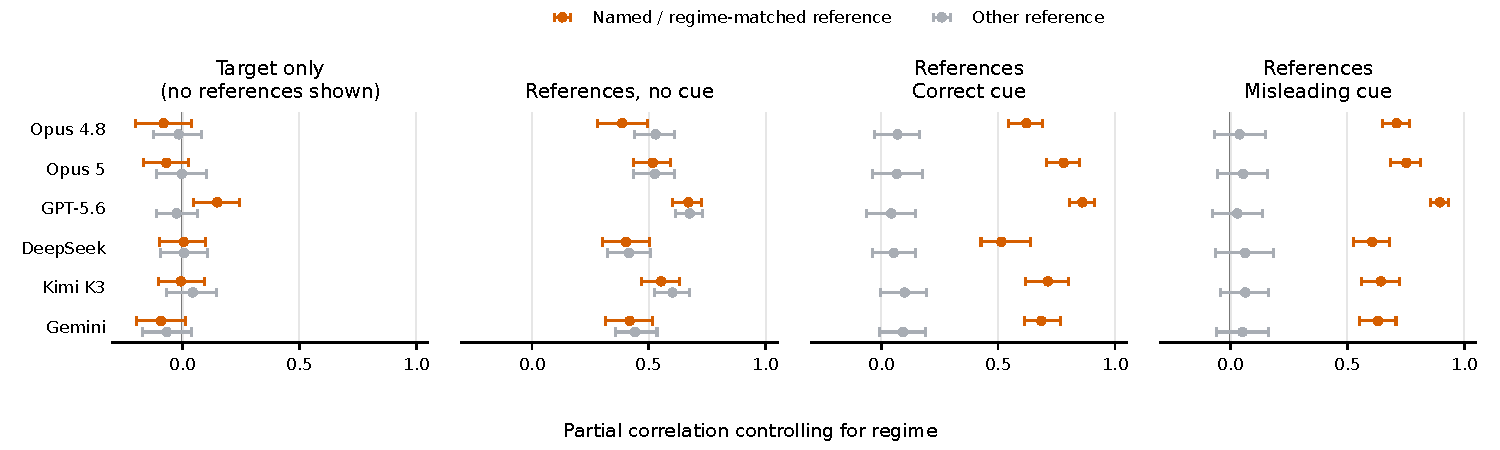
\includegraphics[width=\linewidth]{figures/exp2_reference_selection.pdf}
\caption{\textbf{Forecasts track the reference selected by the cue.}
Points show \(k=0\) partial correlations between forecast-implied responsiveness and each reference city's fitted responsiveness after controlling for regime.
Whiskers give pointwise 90\% episode-bootstrap intervals.
Without a City C cue, forecasts track both displayed references.
Correct and misleading cues concentrate the association on the reference selected by the cue.}
\label{fig:coin-city-reference-selection}
\end{figure}

Without reference-city observations, the corresponding associations are near zero.
When both references are displayed but City C receives no cue, all six primary deployments are positively associated with both reference estimates.
A correct City C cue concentrates this association on the regime-matched reference, with all six named-reference intervals excluding zero and all six other-reference intervals spanning zero.
A misleading cue produces the same pattern for the incorrectly selected reference.
Forecasts therefore depend on reference-specific numerical variation that cannot be explained by a response determined solely by the semantic cue.

The same test under arbitrary labels gives concordant results.
Twelve of fifteen models have positive symbol-matched reference correlations whose 90\% intervals exclude zero.
The three exceptions are Qwen3-4B, Qwen3-8B, and Llama-3.1-8B, which are also the three models whose behavioral symbol-minus-no-context slope-correlation intervals span zero.
Because the behavioral and reference-selection analyses use the same forecasts, this agreement is complementary evidence rather than an independent replication.

The partial correlation measures association with a reference estimate rather than the weight assigned to that estimate.
Shrinking a noisy reference slope toward a regime-level estimate can preserve its residual correlation, so positive values do not imply inefficient transfer of reference noise.
Conversely, a null association does not establish reliance on a lexical prior.
The analysis therefore supports numerical reference selection without identifying the model's internal estimator.

\subsection{Representation and causal analyses}
\label{app:coin-city-mechanistic-probe}

The behavioral analyses establish that some models infer and use an episode-specific reference mapping, but they do not identify how that mapping is represented internally.
We therefore test whether the target regime is linearly decodable from model activations and whether intervening on label-position states changes the resulting forecast.

\subsubsection{Linear-probe methodology}

For each prompt, we extract the hidden state at the final input token from the embedding layer and every transformer block.
Separate ridge probes are fit for each layer, target, and evidence depth using development episodes only.
Features are standardized on the fitting data, and four-fold cross-validation selects both the ridge penalty and probe layer before evaluation on held-out episodes.
No test performance is used for layer or regularization selection.

The probe targets are the binary strong-versus-weak regime, the realized response coefficient \(g_C\), and the within-regime residual
\[
g_C-\mu_{R_e},
\]
where \(\mu_{R_e}=.90\) for the strong regime and \(.25\) for the weak regime.
Regime decoding is scored by ROC AUC, while continuous targets use \(R^2\).
Mean-pooled input embeddings provide a control for information already linearly available from the prompt before transformer processing.

One-sided permutation tests evaluate held-out probe performance with 10,000 target-label permutations while keeping predictions, fitted weights, selected layer, and regularization fixed.
The tests are reported individually without correction across models, targets, or evidence depths.

\paragraph{Why arbitrary labels are the informative probe condition.}

Semantic descriptions explicitly identify City C as belonging to the national or local regime.
Accordingly, the semantic regime is highly linearly decodable even from input embeddings, and high semantic-cue probe performance does not by itself demonstrate an induced internal relationship.
The arbitrary-label condition provides the stronger test because the meanings of \texttt{KIV} and \texttt{ZOR} reverse across episodes and must be inferred from the displayed reference examples.
The larger-sample arbitrary-label probes and causal interventions below therefore carry the primary representational claim.

\subsubsection{Probe targets and information limits}
\label{app:coin-city-probe-ceilings}

The probe analysis distinguishes regime identification from recovery of City C's exact response coefficient.
Under the data-generating process, knowing the true regime mean explains approximately $.992$ of the variance in \(g_C\), because the within-regime standard deviation is only $.03$.
By contrast, City C's within-regime residual is independent of the reference observations at \(k=0\), giving population \(R^2=0\), and four City C observations provide only a small amount of residual information, with an approximate benchmark of \(R^2=.009\).
High full-slope \(R^2\) can therefore arise almost entirely from identifying the response regime.
We consequently treat regime decoding as the primary representational endpoint and use the residual target only as a specificity check.

Under arbitrary labels, comparing the fitted slopes of the two reference cities identifies the target regime with simulated AUC $.979$.
This value describes one estimator available from the displayed examples rather than an optimal ceiling over all possible estimators.

\subsubsection{Arbitrary-label regime decoding}
\label{app:coin-city-probe-power}

The larger probe evaluation uses 248 episodes, with 160 development episodes and 88 held-out test episodes.
Each episode is rendered at \(k=0\) and \(k=4\) under correct, absent, and misleading arbitrary-label assignments.
All seven arbitrary-label models use the same train--test split.
Probe layers and ridge penalties are selected using development episodes only, and the held-out episodes are not used for fitting or model selection.

At \(k=0\), the input embeddings themselves provide little linear information about the arbitrary mapping, with mean-pooled embedding AUCs between $.495$ and $.556$ across the seven models.
After transformer processing, four models show significant held-out regime decoding: Qwen3-14B, Qwen2.5-32B, Qwen2.5-72B, and Llama-3.1-70B.
The remaining three models, Qwen3-4B, Qwen3-8B, and Llama-3.1-8B, do not show significant \(k=0\) regime decoding.

\begin{center}
\begin{minipage}{0.90\linewidth}
\centering
\captionof{table}{\textbf{Zero-shot decoding of an induced arbitrary-label regime.}
Probe AUC is held-out regime decoding at \(k=0\); Embed.\ is the corresponding mean-pooled input-embedding AUC.
The \(p\)-value is from a one-sided 10,000-permutation test.
Behavioral \(\Delta\rho\) is the symbol-minus-no-context slope-correlation effect from Table~\ref{tab:coin-city-symbol-context}.}
\label{tab:coin-city-probe-power}
\small
\begin{tabular}{lrrrr}
\toprule
Model & Probe AUC & Embed. AUC & \(p\) & Behavioral \(\Delta\rho\) \\
\midrule
Qwen3-4B & .520 & .498 & .376 & .095 \\
Qwen3-8B & .566 & .534 & .147 & .023 \\
Qwen3-14B & .678 & .555 & .0016 & .398 \\
Qwen2.5-32B & .778 & .550 & \(<.001\) & .372 \\
Qwen2.5-72B & .662 & .556 & .0026 & .381 \\
Llama-3.1-8B & .423 & .539 & .893 & .045 \\
Llama-3.1-70B & .728 & .495 & \(<.001\) & .424 \\
\bottomrule
\end{tabular}
\end{minipage}
\end{center}

The same four models with significant \(k=0\) regime probes also have behavioral symbol-minus-no-context \(\Delta\rho\) intervals excluding zero.
The other three models have behavioral intervals spanning zero.
This cross-check links linear decodability with behavioral use of the induced convention across checkpoints, although the two analyses use related tasks and are not independent replications.

Qwen3-14B illustrates how the representation changes when direct City C evidence becomes available.
At \(k=0\), its arbitrary-label probe has AUC $.678$ under the correct label, compared with $.467$ with no label and $.321$ under the misleading label.
At \(k=4\), the misleading-arm probe instead favors the true regime, with AUC $.747$, indicating that direct target observations can displace the initially supplied mapping.
This does not imply that all influence of the label disappears.

The checkpoint pattern should not be interpreted as a universal scale threshold.
Within Qwen3, the \(k=0\) effect is detected at 14B but not at 4B or 8B, while Llama-3.1 differs between 8B and 70B.
Model size also changes architecture and training, and the robustness population in Section~\ref{app:coin-city-robustness} changes which individual Qwen3 intervals exclude zero.

\subsubsection{Causal intervention on label-position states}
\label{app:coin-city-causal-patch}

Linear decoding does not establish that the decoded information influences the forecast.
We therefore intervene on the hidden states at the two City C label-token positions under arbitrary labels.
Correct-label and swapped-label prompts are token-aligned and differ only in City C's label.
For each recipient prompt, the intervention replaces the label-position states with the corresponding states from the opposite-label donor and then generates the forecast greedily.

For episode \(e\), let \(s_e=+1\) for a strong-response City C and \(s_e=-1\) for a weak-response City C.
The symmetric intervention effect is
\[
d_e
=
\frac{s_e}{2}
\left[
\left(
\widehat g_{W\leftarrow C,e}
-
\widehat g_{W,e}
\right)
+
\left(
\widehat g_{C,e}
-
\widehat g_{C\leftarrow W,e}
\right)
\right],
\]
where \(C\) and \(W\) denote the correct- and swapped-label prompts and the arrow denotes transfer from donor to recipient.
Positive \(d_e\) means that replacing the recipient state moves its forecast toward the donor label's response regime.

An initial held-out analysis of Qwen3-14B selected transformer outputs 19--21 using probe performance on 160 development episodes and obtained a \(k=0\) mean shift of $.333$ with a 90\% bootstrap interval of \([.198,.471]\) on 88 test episodes.
The selected window produced no positive average shift at \(k=4\).
Because intervention-window selection can itself introduce researcher degrees of freedom, the primary evidence below uses a fresh confirmation set with the window fixed before any new episodes are generated.

\subsubsection{Fixed-window confirmation on fresh episodes}
\label{app:coin-city-fixed-window}

The confirmation uses 88 new episodes from the unchanged generator, balanced across reference-city regime, City C regime, and arbitrary label.
None overlaps the development or test episodes used above.
Before evaluating these episodes, the intervention windows, hypotheses, statistical tests, multiplicity correction, and validity criteria were fixed.

Both Qwen3-14B and Llama-3.1-70B are evaluated at transformer outputs 19--21 and at a later comparison window.
For Qwen3-14B, outputs 19--21 were selected on the preceding 160-episode development set.
For Llama-3.1-70B, outputs 19--21 were chosen from a partial development sweep as a representative location on a broad intermediate-depth plateau rather than as the maximum observed effect.
The late comparison windows are outputs 33--35 for Qwen3-14B and 35--37 for Llama-3.1-70B.

The primary hypotheses are that the mean \(d_e\) at outputs 19--21 is positive at \(k=0\) and that this effect exceeds the corresponding late-window effect.
Tests use one-sided episode-level sign flips with 200,000 draws, with the four primary tests Holm-corrected at familywise level $.05$.
Intervals use 10,000 episode-bootstrap resamples.
Pre-specified validity gates require at least 77 of 88 complete episodes and at least 319 of 352 self-patched forecasts to reproduce their unpatched counterparts exactly.
Both models satisfy both gates.

\begin{center}
\begin{minipage}{\linewidth}
\centering
\captionof{table}{\textbf{Fixed-window intervention on 88 fresh episodes.}
Shift is the mean symmetric effect \(d_e\) in slope units, with 90\% episode-bootstrap intervals.
Positive values indicate movement toward the donor label's regime.
The late window is outputs 33--35 for Qwen3-14B and 35--37 for Llama-3.1-70B.}
\label{tab:coin-city-fixed-window}
\small
\begin{tabular}{l c rr rr}
\toprule
& & \multicolumn{2}{c}{Qwen3-14B} & \multicolumn{2}{c}{Llama-3.1-70B} \\
\cmidrule(lr){3-4}
\cmidrule(lr){5-6}
Patch site & \(k\) & Shift [90\% CI] & \(p\) & Shift [90\% CI] & \(p\) \\
\midrule
Outputs 19--21 & 0 & $.452$ $[.343,.562]$ & \(<5\times10^{-6}\) & $.641$ $[.503,.778]$ & \(<5\times10^{-6}\) \\
Outputs 19--21 & 4 & $-.016$ $[-.094,.059]$ & $.634$ & $.074$ $[.021,.129]$ & $.012$ \\
Late window & 0 & $.044$ $[.010,.082]$ & $.022$ & $-.013$ $[-.026,-.001]$ & $.955$ \\
19--21 minus late & 0 & $.376$ $[.280,.475]$ & \(<5\times10^{-6}\) & $.654$ $[.516,.792]$ & \(<5\times10^{-6}\) \\
\bottomrule
\end{tabular}
\end{minipage}
\end{center}

Both pre-specified \(k=0\) hypotheses are supported for both models after Holm correction.
Patching outputs 19--21 shifts the implied response coefficient toward the donor label's regime by $.452$ in Qwen3-14B and $.641$ in Llama-3.1-70B.
The intermediate-minus-late contrasts are $.376$ and $.654$, respectively, showing that the effect is substantially larger at the selected intermediate depth than at the late comparison window.

Replacing the input embeddings at the label positions produces \(k=0\) shifts of $.528$ for Qwen3-14B and $.665$ for Llama-3.1-70B.
Thus, changing only three intermediate label-position states transfers most of the effect produced by replacing the label representation at the input.

With four City C observations, the Qwen3-14B intermediate-window effect is indistinguishable from zero.
Llama-3.1-70B retains a smaller positive effect of $.074$, indicating that direct target evidence reduces but does not uniformly eliminate reliance on the label.
The experiment therefore supports a causal role for label-position states in zero-shot regime selection while also showing that their influence changes as direct evidence accumulates.

\subsubsection{Interpretation and scope}

The arbitrary-label probes establish linear decodability of an episode-specific mapping in four of seven tested open-weight checkpoints.
The causal interventions go further by showing that replacing label-position states changes zero-shot forecasts in Qwen3-14B and Llama-3.1-70B on fresh episodes.

These interventions replace complete hidden-state vectors rather than a single decoded direction.
They therefore do not establish that the linear probe identifies the unique causal representation, that one representation fully mediates the behavioral effect, or that the same mechanism operates in hosted models.
The causal evidence is restricted to two checkpoints from two model families and one intermediate-depth intervention.

Finally, the task asks models to select between two well-separated response regimes.
It does not test continuous contextual variables or fine-grained recovery of City C's within-regime deviation.
Regime identification, reference selection, and exact coefficient estimation remain distinct capabilities.

\subsection{Robustness across generator populations and deployments}
\label{app:coin-city-robustness}

\subsubsection{Harder generator population}

We repeat the arbitrary-label evaluation on 250 new episodes with strong and weak regime means of $.75$ and $.40$ and within-regime slope standard deviation $.10$.
This jointly reduces between-regime separation and increases within-regime heterogeneity relative to the original population.
Observation noise, factorial balance, prompts, evidence depths, checkpoint settings, and episode-randomized symbol mappings are otherwise unchanged.
Ten open-weight models are evaluated under no City C context, semantic context, and arbitrary-label context at all five evidence depths.

\begin{center}
\begin{minipage}{0.90\linewidth}
\centering
\captionof{table}{\textbf{Zero-shot arbitrary-label effects across generator populations.}
Values are symbol-minus-no-context changes in slope correlation at \(k=0\), with pointwise 90\% episode-bootstrap intervals.
The harder population narrows regime separation and increases within-regime dispersion.}
\label{tab:coin-city-generator-robustness}
\small
\begin{tabular}{lcc}
\toprule
Model & Original \(\Delta\rho\) [90\% CI] & Harder \(\Delta\rho\) [90\% CI] \\
\midrule
Qwen3-4B & $+.095$ $[-.037,.215]$ & $+.050$ $[-.058,.178]$ \\
Qwen3-8B & $+.023$ $[-.105,.146]$ & $+.231$ $[.101,.345]$ \\
Qwen3-14B & $+.398$ $[.276,.520]$ & $+.155$ $[.023,.281]$ \\
Qwen3-32B & $+.302$ $[.201,.410]$ & $+.193$ $[.085,.301]$ \\
Qwen2.5-7B & $+.264$ $[.137,.385]$ & $+.149$ $[.030,.259]$ \\
Qwen2.5-14B & $+.236$ $[.128,.336]$ & $+.133$ $[.026,.233]$ \\
Qwen2.5-32B & $+.372$ $[.255,.488]$ & $+.247$ $[.131,.361]$ \\
Qwen2.5-72B & $+.381$ $[.269,.488]$ & $+.336$ $[.226,.444]$ \\
Llama-3.1-8B & $+.045$ $[-.097,.216]$ & $-.077$ $[-.193,.056]$ \\
Llama-3.1-70B & $+.424$ $[.330,.525]$ & $+.242$ $[.139,.347]$ \\
\bottomrule
\end{tabular}
\end{minipage}
\end{center}

Seven of ten models have positive intervals excluding zero in both populations, and nine of ten retain the same interval classification.
All four Qwen2.5 checkpoints remain positive in the harder population, while Llama-3.1-8B spans zero in both populations and Llama-3.1-70B is positive in both.
Within Qwen3, the checkpoints whose intervals exclude zero change across populations.
The results therefore support robustness of arbitrary-label induction to this joint generator perturbation without implying a universal capability threshold in parameter count.

Forecast discrimination and numerical accuracy remain distinct.
For example, Qwen2.5-72B improves slope discrimination in the harder population while arbitrary-label context increases its forecast MAE by \(1.012\) poll points with a 90\% interval of \([.760,1.271]\).
The harder population changes regime separation and within-regime dispersion simultaneously, so it does not identify the effect of either factor in isolation.

\subsection{Response validity and scope}
\label{app:coin-city-limitations}

\subsubsection{Missing forecasts}

The primary evaluation contains 22,500 model--prompt combinations, of which three lack a usable forecast.
Matched primary comparisons therefore use \(n=249\) for the affected model--prefix combinations and \(n=250\) elsewhere.
All 7,500 misleading-context tasks yield usable analyzed forecasts after deduplication.

The 15-model arbitrary-label comparison contains 56,250 model--prompt combinations and uses complete cases across the three compared conditions.
At \(k=0\), every model contributes 250 complete episodes except Llama-3.1-8B, which contributes 242.
Across later evidence levels, its complete-case sample ranges from 238 to 246.
Unusable forecasts remain missing rather than being imputed.

\subsubsection{Interpretation and scope}

Experiment~2 provides convergent evidence for context-sensitive relationship selection.
Matched cue interventions show that changing only City C's contextual assignment changes the inferred response relationship.
Arbitrary labels show that this assignment can be induced from episode-specific examples rather than supplied by familiar semantics.
Reference-selection analyses show that forecasts track numerical variation in the reference selected by the cue.
Linear probes show that the induced arbitrary-label regime is decodable in several open-weight checkpoints, and the fixed-window interventions show that label-position states causally influence zero-shot forecasts in Qwen3-14B and Llama-3.1-70B.

These analyses answer different questions and are not statistically independent replications.
Behavioral contrasts measure forecast changes, reference-selection correlations measure association with displayed numerical examples, probes measure accessibility to a linear readout, and patching measures the causal effect of replacing selected hidden states.
None identifies a unique internal algorithm.

The scoring target is City C's noise-free conditional expectation rather than a future noisy poll realization.
The prompts explicitly state within-city stability and the matched-pair structure, and the contextual variable is binary and well separated.
The experiment therefore does not establish performance under ambiguous, continuous, or adversarial contextual relationships.

Cross-model comparisons are descriptive because deployments differ in provider, reasoning configuration, and output budget.
The two generator populations jointly vary regime separation and within-regime heterogeneity.
Except where explicitly corrected in the fixed-window causal confirmation, reported bootstrap and permutation intervals are pointwise and do not provide simultaneous coverage across the many models, metrics, and evidence levels.
\clearpage

\section{Experiment 3: controlled relationship transfer}
\label{app:exp3}

Experiment~3 asks whether outcome-based training improves use of an episode-specific response relationship when the forecasting domain or response mechanism changes.
Training uses direct-response systems in Coin City, while evaluation independently varies the surface domain, response mechanism, and amount of target-specific evidence.
The primary comparison holds training prompts and the distribution of reward targets fixed while changing whether each prompt is paired with its own episode-specific target.
Qwen3-4B and Qwen3-8B are each evaluated with eight training seeds per reward arm.

\subsection{Design and evaluation}
\label{app:exp3-coin-structural}

\subsubsection{Domains and response mechanisms}
\label{app:exp3-domain-contrast}

Let \(x_t\) denote the input and \(z_t\) the latent deviation of the outcome from its resting level.
Training uses the direct-response mechanism,
\begin{equation}
z_{t+1}=g_jx_t.
\label{eq:exp3-coin-a}
\end{equation}
A pulse therefore affects the next observation but does not persist after subsequent inputs return to zero.

Evaluation additionally includes a mediated mechanism,
\begin{align}
m_{t+1}&=\rho m_t+g_jx_t,\\
z_{t+1}&=\phi z_t+\lambda m_{t+1}.
\label{eq:exp3-coin-b}
\end{align}
Both latent states begin at zero.
Observed outcomes add independent Gaussian noise and are clipped to the stated domain range, while evaluation targets use the corresponding noise-free trajectory.
Prompts provide the domain bounds and qualitative pathway descriptions but omit the equations, response parameters, mediator, and structure labels.

Coin City has resting level \(50\), support \([0,100]\), and observation-noise standard deviation \(1.6\).
Coin Harbor changes the terminology, units, numerical scale, input magnitudes, and pathway descriptions, with resting level \(180\), support \([40,320]\), and observation-noise standard deviation \(4.5\).
Training reference gains are sampled from \([.18,.46]\) for the weak-response system and \([.68,.98]\) for the strong-response system.
At evaluation, \(g\sim\mathrm{Uniform}(.22,.92)\), while Structure~B uses \(\rho\sim\mathrm{Uniform}(.48,.74)\), \(\phi\sim\mathrm{Uniform}(.18,.42)\), and \(\lambda\sim\mathrm{Uniform}(.68,.94)\).
Coin City inputs are drawn from \(\{-12,-8,-4,0,4,8,12\}\), while Coin Harbor uses \(\{-24,-16,-8,0,8,16,24\}\).
Evaluation queries use shocks \(\{-12,-6,0,6,12\}\) in Coin City and \(\{-24,-12,0,12,24\}\) in Coin Harbor at horizons one and three.
A reference and its matched target share these latent response parameters but have independent inputs and observation noise.

\begin{center}
\begin{minipage}{0.90\linewidth}
\centering
\captionof{table}{\textbf{Training and transfer conditions.} Training uses Coin City with the direct response mechanism, while evaluation independently changes the surface domain and response structure.}
\label{tab:exp3-domain-contrast}
\small
\begin{tabular}{lll}
\toprule
Evaluation cell & Domain & Response structure \\
\midrule
In distribution & Coin City & Direct, Structure~A \\
Domain shift & Coin Harbor & Direct, Structure~A \\
Structure shift & Coin City & Mediated, Structure~B \\
Joint shift & Coin Harbor & Mediated, Structure~B \\
\bottomrule
\end{tabular}
\end{minipage}
\end{center}

\subsubsection{Episode-matched training and population-prior control}

Each training prompt contains two complete 14-case reference systems with different response gains and a target that shares one reference's gain.
The target reveals \(k\in\{0,2,4,8\}\) observations, and its qualitative background identifies the matching response regime.
Training contains 1,200 prompts at each evidence depth, for 4,800 prompts in total.
Weak- and strong-response targets are balanced overall but associated with evidence depth, so \(k\) itself provides some information about the gain band.

The episode-matched and population-prior conditions receive identical prompts and the same multiset of answer vectors.
Episode-matched reward scores a response against the forecasts generated by that episode's own latent parameters.
The population-prior control reassigns complete answer vectors among episodes with the same evidence depth so that every vector is used exactly once and no episode retains its own vector.
This preserves the reward distribution conditional on \(k\) while removing the episode-specific prompt--target pairing.
The contrast therefore tests episode-specific supervision beyond learning the answer distribution associated with evidence depth and other shared prompt features.

\paragraph{Training reward and output contract.}

The Experiment~3 reward is
\[
r=.4\,r_{\mathrm{level}}+.6\,r_{\mathrm{response}},
\]
where each component averages \(\max(0,1-|e|/S)\) over its corresponding forecast errors.
The level tolerance is 10\% of the domain's observable range, while the response tolerance is half one intervention unit.
Training and evaluation require exactly ten finite forecasts in a JSON object; malformed or length-truncated outputs receive zero training reward.

\subsubsection{Evaluation protocol}

Every evaluation prompt contains one complete direct-response reference, one complete mediated-response reference, and a target generated by one of those mechanisms.
The target receives either the correct qualitative pathway description, no pathway description, or the description of the other mechanism.
These prompt variants reuse exactly the same numerical observations and forecast queries.

Each task requests ten counterfactual forecasts spanning five intervention magnitudes and horizons one and three.
Response error is computed from the eight nonzero-shock responses after subtracting the corresponding zero-shock forecast at each horizon.
Evaluation crosses two domains, two response structures, three hint conditions, four target-evidence depths, and 30 episodes, for 1,440 prompts per checkpoint.

The primary contrast is population-prior minus episode-matched response MAE under the correct pathway description.
Positive values favor episode-matched training.
The four evaluation cells measure performance in distribution, under domain shift, under structure shift, and under both shifts jointly.

All reported endpoints use round 300 and five stochastic forecasts per prompt at temperature \(0.7\).
Each forecast draw is scored separately before averaging within a prompt.
Invalid forecasts receive an error equal to the observable range of the corresponding domain.

\subsection{Eight-seed transfer results}
\label{app:exp3-eight-seed}

Qwen3-4B and Qwen3-8B are each evaluated with eight training seeds per reward arm, using seeds 42--49.
The data, 300-round endpoint, five-draw decoder, and transfer estimands are shared across the two reward conditions.
The hierarchical bootstrap first resamples training seeds and then paired evaluation prompts within each selected seed.
Brackets give 90\% hierarchical bootstrap intervals. We additionally summarize seed-level uncertainty with a two-sided wild-cluster bootstrap with Webb weights and an exact one-sided sign test.

The eight-seed roster is a precision extension rather than the prospectively fixed seed count of the initial study.
The endpoint, training data, decoder, estimands, and added-seed analysis procedures were fixed for the extension before the added endpoints were available.
Because the decision to increase the seed count followed an earlier analysis, we interpret the eight-seed results as precision estimates rather than as a fully prospective confirmatory test.

\begin{center}
\begin{minipage}{0.82\linewidth}
\centering
\captionof{table}{\textbf{Eight-seed population-prior minus episode-matched response MAE.} Positive values favor episode-matched training, and brackets give hierarchical 90\% intervals. All cells use the correct pathway description and average the four evidence depths equally.}
\label{tab:exp3-transfer-summary}
\small
\begin{tabular}{lcc}
\toprule
Evaluation cell & Qwen3-8B & Qwen3-4B \\
\midrule
In distribution & $.060$ $[.023,.103]$ & $.067$ $[-.037,.171]$ \\
Domain shift & $.110$ $[-.006,.242]$ & $.087$ $[-.061,.232]$ \\
Structure shift & $-.003$ $[-.046,.035]$ & $.052$ $[-.055,.159]$ \\
Joint shift & $.126$ $[.018,.242]$ & $.136$ $[-.005,.275]$ \\
\bottomrule
\end{tabular}
\end{minipage}
\end{center}

For Qwen3-8B, episode-matched training has lower point-estimate error in distribution, under domain shift, and under joint shift, while the structure-shift contrast is approximately zero.
The in-distribution and joint-shift contrasts have hierarchical intervals excluding zero; the domain-shift and structure-shift intervals include zero.
The in-distribution contrast is also supported by the wild-cluster test, \(p=.0089\), and by eight positive seed-level effects out of eight.
The corresponding one-sided exact sign-test value is \(p=.0039\).

The Qwen3-8B joint-transfer contrast is $.126$ with hierarchical interval \( [.018,.242] \).
The interval excludes zero, but the wild-cluster test gives \(p=.091\) and six of eight seed-level effects are positive, so the estimate remains compatible with a small advantage from episode-matched supervision rather than a large one.
The domain-shift interval likewise includes zero, while the structure-shift estimate is centered near zero.

For Qwen3-4B, all four hierarchical intervals include zero.
Its point estimates are positive in every evaluation cell, but the eight-seed data do not distinguish these effects from zero under the reported hierarchical intervals.

Taken together, the eight-seed results provide evidence that episode-specific supervision improves Qwen3-8B performance on the response relationship seen during training.
They provide weaker evidence that this advantage transfers under a new domain or a new response mechanism alone; under joint shift the hierarchical interval excludes zero, but the wild-cluster test and the six-of-eight seed count do not support a clear effect.
The results therefore distinguish learning the episode-specific training relationship from robust transfer of that relationship under structural change.

\subsection{Exploratory diagnostics of relationship learning}

The eight-seed experiment above evaluates whether episode-specific supervision improves transfer.
The following diagnostics ask a narrower question: when transfer fails, is the underlying response relationship learnable, and does training make forecasts track episode-specific evidence rather than only a population-level target distribution?
These analyses use separate experimental rosters and are not part of the primary eight-seed transfer comparison.

\subsubsection{Supervised learnability and its transfer boundary}
\label{app:exp3-learnability}

We first ask whether the response-structure task is learnable from direct supervision.
This diagnostic uses a separate structure-selection dataset in which every prompt contains one direct and one mediated reference.
Their horizon-one response magnitudes are matched, while their horizon-three persistence differs, so selecting the correct response form requires distinguishing temporal structure rather than immediate response magnitude.
Targets are balanced equally between the two structures.
Qwen3-8B is fine-tuned on 4,800 such Coin City prompts using simulator-correct forecasts as targets.
The higher-rate supervised recipe uses learning rate \(2\times10^{-5}\), one epoch, 300 updates, and four independent training seeds.
Neither Coin Harbor nor arbitrary labels appears during training.

Across the four seeds, in-distribution Coin City forecasts identify the correct response structure on \(97.9\%\)--\(100.0\%\) of prompts, with response MAE between $.277$ and $.658$.
The same models remain near the binary-choice baseline when the relationship must transfer to arbitrary labels or Coin Harbor.
City/arbitrary accuracy ranges from \(39.6\%\) to \(50.0\%\), Harbor/semantic from \(45.8\%\) to \(52.1\%\), and Harbor/arbitrary from \(47.9\%\) to \(50.0\%\).
Reference identification remains \(100\%\) throughout.

The supervised result establishes that the in-distribution response-form selection problem is learnable by this model and recipe.
Its failure under arbitrary labels and domain transfer shows that successful in-domain structure selection does not imply inference of the response relationship from unfamiliar reference examples.
This is not a controlled SFT-versus-RL comparison because the objectives, learning rates, and effective training budgets differ.

\subsubsection{Mechanism-family evidence use under coherent gain changes}
\label{app:exp3-evidence-use}

This diagnostic uses a separate Qwen3-4B mechanism-family training study with eight response mechanisms represented during training and four held out for evaluation.
Episode-matched and shuffled-target models use the same mechanism-balanced prompts and training budget; the shuffled arm preserves the answer-vector distribution within compatible mechanism and evidence-depth groups while breaking the episode-specific pairing.
We test whether trained forecasts track an episode-specific change in response strength.
The diagnostic contains 16 paired episodes from each of 12 response mechanisms, comprising eight mechanisms represented during training and four held-out compositions or parameter-extrapolation mechanisms.
Both mechanism-disclosed and mechanism-undisclosed conditions use the same episodes and nine target observations.

Within each pair, the target gain changes from the 20th to the 80th percentile of that mechanism's gain distribution.
Inputs, observation-noise draws, reference trajectories, baseline state, and mechanism remain fixed, while target observations and forecast outcomes are recomputed under the new gain.
The disclosed description states the same gain range for both members and never reveals the realized gain.

Let \(\Delta r_i\) denote the simulator's change in the eight-coordinate response vector between the high- and low-gain episodes, and let \(\Delta\widehat r_i\) denote the corresponding predicted change.
We measure
\[
E_{\Delta}
=
\frac{1}{8N}
\sum_{i=1}^{N}
\left\|
\Delta\widehat r_i-\Delta r_i
\right\|_1,
\qquad
\beta_{\Delta}
=
\frac{\sum_i\Delta\widehat r_i^\top\Delta r_i}
{\sum_i\lVert\Delta r_i\rVert_2^2}.
\]
Exact tracking gives \(\beta_{\Delta}=1\), while a forecast invariant to the gain change gives zero.

The comparison uses five training seeds per arm of episode-matched and distribution-matched shuffled-target training.

\begin{center}
\begin{minipage}{\linewidth}
\centering
\captionof{table}{\textbf{Episode-specific gain tracking on seen and held-out mechanisms.}
Entries are response-change MAE, with lower values better.
Slope M and S are the tracking slopes for episode-matched and shuffled-target training.
Positive shuffled-minus-matched contrasts favor episode matching. Brackets give 90\% intervals from 2,000 seed-then-episode bootstrap repetitions.}
\label{tab:exp3-gain-evidence}
\footnotesize
\setlength{\tabcolsep}{3pt}
\begin{tabular}{llrrrrrr}
\toprule
Disclosure & Set & Matched & Shuffled & \shortstack{No\\change} & \shortstack{Slope\\M} & \shortstack{Slope\\S} & \shortstack{Shuffled\\\(-\) matched} \\
\midrule
Disclosed & Seen     & 1.250 & 1.512 & 1.591 & .323 & .084 & \(+.262\) \([+.220,+.308]\) \\
Disclosed & Held out & .898  & .874  & .826  & .122 & .049 & \(-.024\) \([-.069,+.019]\) \\
Undisclosed & Seen     & 1.115 & 1.488 & 1.591 & .461 & .107 & \(+.373\) \([+.326,+.418]\) \\
Undisclosed & Held out & .878  & .862  & .826  & .238 & .060 & \(-.016\) \([-.055,+.020]\) \\
\bottomrule
\end{tabular}
\end{minipage}
\end{center}

Episode-matched training improves tracking on mechanisms represented during training.
The response-change MAE advantage is $.262$ with mechanism disclosure and $.373$ without disclosure, with both intervals excluding zero.
The corresponding matched tracking slopes, $.323$ and $.461$, are also substantially larger than those of the shuffled control.

This advantage does not extend to the held-out mechanisms.
The shuffled-minus-matched contrasts are \(-.024\) and \(-.016\), and both intervals include zero.
Moreover, the episode-matched held-out errors exceed the $.826$ no-change baseline despite positive tracking slopes of $.122$ and $.238$.
The models therefore respond to held-out gain changes without accurately tracking them.
Improved accuracy on familiar mechanisms does not establish transferred episode-specific evidence use.

\subsubsection{Distribution-matched shuffled-target control}
\label{app:exp3-shuffled-control}

The shuffled-target control addresses a limitation of the population-prior comparison in the primary experiment.
Within compatible mechanism and evidence-depth groups, it preserves the complete multiset of training answer vectors while reassigning those vectors across episodes.
Prompts, training budget, and target distribution are therefore fixed while the episode-specific prompt--target correspondence is removed.

The prospectively fixed comparison uses five training seeds per arm.
Under stochastic decoding with the mechanism undisclosed, the shuffled-minus-matched response-MAE contrast is \(+.094\).
Its 90\% hierarchical interval is \([+.041,+.168]\), the wild-cluster test gives \(p=.0138\), and all five seed-level contrasts are positive.
The corresponding exact one-sided sign test gives \(p=.0312\).

With the mechanism disclosed, the stochastic contrast is \(+.155\), with hierarchical interval \([+.062,+.243]\).
Four of five seeds are positive, while the wild-cluster test gives \(p=.079\).
The distribution-matched control therefore supports an episode-matching advantage in the frozen five-seed undisclosed condition, while the strength of evidence varies across disclosure and inference procedures.

A later sensitivity extension adds three training seeds to each arm.
Because the final seed was added after the seven-seed result was known, these eight-seed estimates are descriptive rather than prospectively calibrated.
On the undisclosed stochastic endpoint, the contrast decreases to \(+.061\), with hierarchical interval \([+.001,+.125]\), wild-cluster \(p=.101\), and six of eight positive seeds.
The interval excludes zero only narrowly, the point estimate is smaller, the wild-cluster test does not reject, and the seed count is weaker than in the five-seed roster, so the extension does not strengthen the evidence beyond the prospectively fixed five-seed comparison.

Taken together, these diagnostics separate three notions of learning.
A supervised model can learn semantic response-form selection in the training domain without transferring that selection to arbitrary labels or a new domain.
Episode-matched training improves tracking of gain changes for mechanisms represented during training but not for held-out mechanisms.
A distribution-matched shuffled-target control provides evidence that episode-specific prompt--target pairing can matter, while the strength of that evidence depends on the evaluation condition and seed roster.
None of these results establishes general transfer of an induced response relationship to unseen mechanisms.

\section{Experiment 4: historical-market training and held-out evaluation}
\label{app:exp4}
\label{app:exp3b-protocol}

Experiment~4 tests whether outcome-based training improves forecasts for events and question families absent from the fine-tuning data.
Models receive a prediction-market question, its resolution rules, and the market-price history available by a fixed forecast cutoff, then predict the probability of YES.
Training uses a Brier-score reward, and evaluation separates markets temporally and by event and question family.

\subsection{Sample construction and leakage controls}

The source archive contains 1,788,703 market records.
The selected datasets contain 1,736 training, 512 development, and 1,024 test markets, with YES rates $.311$, $.275$, and $.301$, respectively.
Training contains 991 distinct events and 1,456 normalized question templates; development contains 292 events and 453 templates; test contains 493 events and 866 templates.

We include binary markets with literal Yes/No outcomes and an archived Boolean resolution inferred from an extreme final token price.
A fixed domain filter retains political, governmental, macroeconomic, and geopolitical questions while excluding sports, entertainment, cryptocurrency, and other out-of-scope categories.
The forecast cutoff is 30 days before the earliest available resolution, market-close, market-end, or event-end timestamp.
Eligible markets require at least four distinct pre-cutoff trading dates, a latest available price no more than seven days old, and a latest YES price in \([.02,.98]\).
Prompts contain at most the latest 14 pre-cutoff YES closing prices together with the question, resolution rules, and cutoff date.
Outcomes, terminal prices, market status, terminal timestamps, volume, and selection metadata are withheld.

Training cutoffs precede July~1, 2025, development cutoffs fall between July~1 and December~31, 2025, and test cutoffs fall between January~1 and June~30, 2026.
Development markets sharing an event, available series identifier, or normalized question template with training are removed, and the same exclusion is then applied to test markets against both earlier splits.
Numeric values and month names are normalized when constructing template keys.
The final train--development, train--test, and development--test family intersections are all empty.

The archive provides timestamped price histories but not historical revisions to static question or resolution-rule text.
We therefore treat those strings as time-invariant.
The design prevents leakage through post-cutoff prices and explicit family reuse, but it cannot establish that historical events were absent from model pretraining.

\subsection{Training and evaluation}

Training uses the 1,736 unique markets in a deterministic 4,800-presentation schedule.
Every market appears at least twice, and the resulting 300 rollout rounds and 2,400 optimizer updates match the training budget used elsewhere in the paper.
Models are optimized directly for Brier reward,
\[
r=1-(\widehat p-y)^2.
\]

\begin{center}
\begin{minipage}{0.88\linewidth}
\centering
\captionof{table}{\textbf{Historical-market training and evaluation configuration.}}
\label{tab:exp3b-hparams}
\small
\begin{tabular}{p{0.34\linewidth}p{0.57\linewidth}}
\toprule
Quantity & Value \\
\midrule
Models & Qwen3-4B-Instruct-2507, Qwen3-8B, Llama-3.1-8B-Instruct \\
Training markets & 1,736 unique markets; 4,800 presentations \\
Training & 300 rounds; seeds 42, 43, 44 \\
Reward & \(1-(\widehat p-y)^2\) \\
Optimization & Dr.~GRPO; AdamW; learning rate \(10^{-6}\) \\
Rollouts & 16 prompts per round; 8 responses per prompt; temperature \(1.3\) \\
Development & 512 markets \\
Held-out evaluation & 1,024 markets; temperature zero; one forecast per market \\
\bottomrule
\end{tabular}
\end{minipage}
\end{center}

Held-out evaluation uses Brier loss.
The reported trained score averages the three seed-specific losses rather than averaging their forecast probabilities.
Invalid forecasts receive Brier loss one.
Pointwise 90\% intervals use 5,000 bootstrap resamples of connected event/template components, preserving markets that belong to the same connected family.
These intervals quantify held-out market-sample variation conditional on the three fitted models.

\subsection{Held-out results}
\label{app:exp3b-results}

All three model families improve relative to their corresponding untrained checkpoints on the 1,024 family-disjoint test markets.

\begin{center}
\begin{minipage}{0.88\linewidth}
\centering
\captionof{table}{\textbf{Held-out historical-market forecasting.}
Trained Brier scores average three training seeds.
Negative trained-minus-base differences favor training, with 90\% family-clustered bootstrap intervals.}
\label{tab:exp4-endpoint-results}
\small
\begin{tabular}{lrrr}
\toprule
Model & Base Brier & Trained Brier & Trained \(-\) base [90\% CI] \\
\midrule
Qwen3-4B & .1316 & .1159 & $-.0157$ $[-.02355,-.00809]$ \\
Qwen3-8B & .1287 & .1164 & $-.0123$ $[-.01825,-.00684]$ \\
Llama-3.1-8B & .1520 & .1150 & $-.0370$ $[-.05095,-.02449]$ \\
\bottomrule
\end{tabular}
\end{minipage}
\end{center}

Every Qwen3-8B training seed improves on its untrained base, and the same base-relative pattern holds for Qwen3-4B and Llama-3.1-8B.
These results establish base-relative improvement on temporally later markets whose event and normalized question families were excluded from fine-tuning.

The latest pre-cutoff market price obtains Brier $.11369$.
A logistic recalibration of its logit, fit using only the training split, obtains Brier $.11232$.
The trained-minus-market interval includes zero for Qwen3-4B, $+.0022$ \( [-.00187,+.00645] \), whereas Qwen3-8B and Llama-3.1-8B have higher error than the market by $+.0027$ \( [+.00038,+.00555] \) and $+.0013$ \( [+.00006,+.00332] \).
Against the recalibrated market benchmark, Qwen3-4B's interval also includes zero, $+.0036$ \( [-.00047,+.00784] \), while Qwen3-8B and Llama-3.1-8B have higher error by $.00409$ \( [.00139,.00714] \) and $.00269$ \( [.00091,.00484] \), respectively.
The historical experiment therefore establishes improvement relative to the models' untrained bases rather than superiority to prediction-market forecasts.

\subsection{Scale comparison}
\label{app:exp4-scale}

A separate 318-market holdout tests how the same training recipe behaves across Qwen3 scale.
These markets have forecast cutoffs between January~1 and June~8, 2026, and their identifiers, events, available series, and normalized question templates are absent from the training, development, and original 1,024-market test sets.
The holdout contains 227 event families and 288 normalized templates, and selection does not use outcomes or market probabilities.

Qwen3 checkpoints from 1.7B through 32B use the same training data, three seeds, 4,800-presentation schedule, reward, and development rule.
Each base and trained checkpoint receives five non-thinking forecasts per market at temperature $.7$, top-\(p=.8\), and top-\(k=20\).
Forecast probabilities are averaged within each five-draw group before computing Brier loss.
All Qwen3 draws parse successfully.

\begin{center}
\begin{minipage}{0.82\linewidth}
\centering
\captionof{table}{\textbf{Qwen3 scale comparison on the 318-market holdout.}
Trained means average seeds 42--44, and lower Brier is better.}
\label{tab:exp4-qwen-scale-results}
\small
\begin{tabular}{lrrr}
\toprule
Checkpoint & Base & Trained mean & Trained \(-\) base \\
\midrule
Qwen3-1.7B & .2253 & .1248 & $-.1005$ \\
Qwen3-4B-Instruct-2507 & .1522 & .1366 & $-.0156$ \\
Qwen3-8B & .1369 & .1286 & $-.0083$ \\
Qwen3-14B & .1281 & .1270 & $-.0012$ \\
Qwen3-32B & .1266 & .1265 & $-.0001$ \\
\bottomrule
\end{tabular}
\end{minipage}
\end{center}

The base-relative gain decreases as the untrained Qwen3 checkpoint improves.
At 32B, trained-minus-base is \(-.00007\) with a 90\% interval of \([-.00039,+.00023]\).
The 14B trained model has lower Brier than the 8B trained model by $.00164$ with interval \([.00043,.00299]\), but the trained 14B and 32B checkpoints are already close in absolute error.

Contemporaneous Polymarket prices obtain Brier $.12655$ on this holdout.
Trained 14B minus market is \(+.00040\) \( [-.00019,+.00122] \), and trained 32B minus market is \(-.00003\) \( [-.00008,+.00002] \).
Both intervals include zero.
Under this fixed training recipe, larger untrained checkpoints approach the absolute performance of the trained models, so increasing parameter count does not imply a larger training gain.

Llama-3.1-8B provides an architecture comparison on the same holdout.
Its trained mean is $.12643$, compared with $.16417$ for the base, for a difference of \(-.03774\) \( [-.05482,-.02230] \).
Its trained-minus-market difference is \(-.00012\) \( [-.00039,+.00009] \).
The Llama result therefore reproduces the pattern of substantial base-relative improvement without establishing lower error than the contemporaneous market.

\paragraph{Hosted-model references.}

DeepSeek V4-Pro, Claude Opus~4.8, GPT-5.6, and Kimi K3 are evaluated on the same 318 markets as external performance references.
Their Brier scores are $.12660$, $.12927$, $.13335$, and $.12682$, respectively, compared with $.12655$ for Polymarket.
Provider sampling and reasoning configurations differ from one another and from the local checkpoints, so these values provide context rather than a controlled model-family or scale comparison.

\subsection{Price ablation: forecasting without market history}
\label{app:exp4-price-ablation}

The historical-market prompts include dated pre-cutoff prices, whose latest value is itself a strong forecast.
To test how much trained performance depends on this information, we evaluate the same trained adapters after removing the entire price-history block while leaving the question, resolution rules, cutoff, and output format unchanged.
Models are not retrained for this ablation.

We report the 1,024-market held-out evaluation for Qwen3-1.7B, Qwen3-14B, and Qwen3-32B.
Each trained value averages seeds 42--44.
The no-price evaluation uses one temperature-zero forecast per market, matching the primary held-out evaluation.
The training-set YES rate of $.311$ provides a fixed climatology benchmark with Brier loss $.21042$.

\begin{center}
\begin{minipage}{0.84\linewidth}
\centering
\captionof{table}{\textbf{Removing market-price history eliminates the held-out accuracy of the trained models.} Brier loss is lower when better. Trained values average three seeds.}
\label{tab:exp4-price-ablation}
\small
\begin{tabular}{lrrr}
\toprule
Model & No-price base & No-price trained & Trained with prices \\
\midrule
Qwen3-1.7B & .2611 & .2468 & .1183 \\
Qwen3-14B & .2381 & .2413 & .1147 \\
Qwen3-32B & .2935 & .2933 & .1151 \\
\bottomrule
\end{tabular}
\end{minipage}
\end{center}

Without price history, every trained model performs worse than the $.21042$ climatology benchmark.
Removing prices raises trained Brier from $.1183$ to $.2468$ at 1.7B, from $.1147$ to $.2413$ at 14B, and from $.1151$ to $.2933$ at 32B.
Training also provides no consistent advantage over the corresponding no-price base models: the 1.7B difference is $-.01429$ with a 90\% interval of $[-.02838,-.00191]$, the 14B difference is $+.00322$ $[+.00097,+.00554]$, and the 32B difference is $-.00020$ $[-.00301,+.00249]$.

The historical-market gains therefore depend strongly on having market-price history available at inference time.
This ablation evaluates models trained with prices and then tested without them, so it does not establish whether training on price-free prompts could produce useful price-free forecasts.

\section{Experiments 3--4: shared training configuration}
\label{app:exp3-complete-training-setup}

Experiments~3 and~4 use the same Dr.~GRPO training implementation unless a study-specific section states otherwise.
Table~\ref{tab:exp3-oat-common} reports the parameters needed to reproduce the shared optimization procedure.

\begin{center}
\begin{minipage}{\linewidth}
\centering
\captionof{table}{\textbf{Shared Dr.~GRPO training configuration.}}
\label{tab:exp3-oat-common}
\small
\begin{tabular}{p{.28\linewidth}p{.66\linewidth}}
\toprule
Quantity & Configuration \\
\midrule
Adaptation & Frozen base model with LoRA rank 32 and $\alpha=64$ on attention and feed-forward projections; bfloat16; no quantization \\
Objective & Dr.~GRPO with group-centered rewards and no group-standard-deviation normalization; PPO clip $.2$; importance-sampling cap $2.0$; one PPO epoch; KL coefficient $0$ \\
Optimizer & AdamW; learning rate $10^{-6}$; $\beta_1=.9$, $\beta_2=.95$; weight decay $0$; maximum gradient norm $1.0$ \\
Batching & 16 prompts per rollout round; 8 sampled responses per prompt; 128 trajectories per round \\
Schedule & 4,800 prompt presentations; 300 rollout-and-update rounds; 2,400 AdamW updates; constant learning rate with no warmup \\
Training decoding & Temperature $1.3$; top-$p=1$; no top-$k$ restriction \\
Invalid outputs & Missing, malformed, or length-truncated required outputs receive reward zero \\
Training seeds & Experiment~3 primary Qwen comparison: seeds 42--49; Experiment~4 historical-market training: seeds 42--44 \\
\bottomrule
\end{tabular}
\end{minipage}
\end{center}

One reported training ``round'' denotes one rollout-and-update cycle over 16 prompts and eight sampled responses per prompt.
With the implemented microbatching and gradient accumulation, each round performs eight AdamW updates, giving 2,400 optimizer updates over 300 rounds.
Study-specific datasets, reward functions, evaluation decoding, and uncertainty procedures are described in their respective experiment sections.
